% Basic setup. Most papers should leave these options alone.
\documentclass[fleqn,usenatbib]{mnras}
\usepackage{newtxtext,newtxmath}
\usepackage[T1]{fontenc}
\usepackage{ae,aecompl}

%%%%% AUTHORS - PLACE YOUR OWN PACKAGES HERE %%%%%
% Only include extra packages if you really need them. Common packages are:
\usepackage{graphicx}	% Including figure files
\usepackage{amsmath}	% Advanced maths commands
\usepackage[para, flushleft]{threeparttable}
\usepackage{hyperref}
\usepackage{natbib}
\usepackage{booktabs}
\usepackage{color}
\usepackage{soul}
\usepackage{fix-cm}
\usepackage{caption}   % Caption is required to avoid errors.

% Own commands
\newcommand{\kmps}{\,kms\(^{-1}\)}	% kilometres per second

\newcommand*\bl{\color{blue}}

\title[Towards the nIR detection of BD companions]{Towards the near-infrared detection of brown dwarf companions: Exploring methods to detect low mass stellar companions from blended spectra \thanks{Based on observations collected at the European Organisation for Astronomical Research in the Southern Hemisphere under ESO programme 089.C-0977(A)}}

\author[J. J. Neal et al.]{
J. J. Neal$^{1,2}$\thanks{E-mail: jason.neal@astro.up.pt}
P. Figueira$^{3,1}$
N. C. Santos$^{1,2}$
C. Melo$^{3}$
\\
% List of institutions
$^{1}$Instituto de Astrof\'{\i}sica e Ci\^encias do Espa\c{c}o, CAUP, Universidade do Porto, Rua das Estrelas, PT4150-762 Porto, Portuga\\l
$^{2}$Departamento de F\'{\i}sica e Astronomia, Faculdade de Ci\^{e}ncias, Universidade do Porto, Portugal\\
$^{3}$European Southern Observatory, Alonso de C\'{o}rdova 3107, Vitacura, Casilla 19001, Santiago 19, Chile\\
}
% These dates will be filled out by the publisher
\date{Accepted XXX. Received YYY; in original form ZZZ}

% Enter the current year, for the copyright statements etc.
\pubyear{2018}

% Don't change these lines
\begin{document}
\label{firstpage}
\pagerange{\pageref{firstpage}--\pageref{lastpage}}
\maketitle

% Abstract of the paper
\begin{abstract}
   {\bl In this paper we attempt to directly detect the near-infrared (nIR) spectrum of candidate brown dwarf (BD) companions around FGK stars to assert or discard their stellar nature. Individual nIR spectra are fitted to a synthetic binary model comprised of two PHOENIX-ACES spectra using a $\chi^2$ approach. The observed spectra are wavelength calibrated and corrected for the atmospheric absorption with the aid of synthetic telluric models. This was unable to successfully detect the faint spectra of even the largest companion in the sample. We explore how the companion recovery fitting performs on simulated observations and discuss reasons for the non-detection observed. From the injection-recovery analysis, this technique in its current form, is insufficient to recover a companion below 3800~K which corresponds to an upper mass limit for the companions around \(\rm 600~M_{Jup}\). This work highlights the challenges in the spectral detection of faint companions. We explore the limitations of the companion detection with synthetic models at low companion/host flux ratios below 1 per cent, made difficult by the discrepancy between observed and synthetic spectra around 2100~nm.}

\end{abstract}

\begin{keywords}
brown dwarfs -- binaries: spectroscopic -- infrared: stars -- techniques: spectroscopic -- methods: miscellaneous
\end{keywords}


\section{Introduction}
\label{sec:intro}
Brown dwarfs (BDs) are sub-stellar objects unable to achieve hydrogen fusion, with masses around \(13-80~\textrm{M}_{Jup}\)~\citep{chabrier_theory_2000}, bridging the gap between low-mass stars and giant planets. Without sustained fusion, brown-dwarfs cool down over time with an age-dependent cooling rate. Therefore, there is an inherent degeneracy between the mass, age and luminosity of a given BD\citep{burrows_nongray_1997}. This degeneracy may be broken by observation of several parameters, for instance when a BD is in a binary system with a main sequence host star, using both the {\bl host stars' age} and the masses derived from the dynamical motion.

A paucity of BD companions exists in short period orbits around Sun-like stars (\(\lesssim5\)\,AU), compared to stellar or planetary companions, termed the \emph{brown dwarf desert}~\citep{halbwachs_exploring_2000,zucker_analysis_2001,sahlmann_search_2011}. As the number of known BDs orbiting solar type stars is low, the characterization of benchmark BDs in the brown dwarf desert~\citep[e.g.][]{crepp_trends_2016} is beneficial in understanding this sub-stellar population and to help constrain formation and evolution theories~\citep{whitworth_formation_2007}. The BD desert also provides a greater challenge as it reduces the amount of good BD candidates to study.

BDs in binary systems, unlike free-floating BDs, allow for the determination of their masses, when complemented with radial velocity (RV) and astrometry measurements. The RV technique provides the mass lower-limit (\(\textrm{M}_{2}\sin{i}\)) of binary and planetary companions, while complementary astrometry measurements can often provide mass upper-limits~\citep[e.g.][]{sahlmann_search_2011}. Measuring or tightening the constraints of BD masses improves the understanding of mass dependence on BD formation processes. For instance, there is growing evidence that the larger giant planets and BD companions do not follow the well known metallicity-giant planet correlation seen in main-sequence stars with planets~\citep[e.g.][]{santos_spectroscopic_2004,santos_observational_2017, maldonado_searching_2017}. Photometry along with stellar evolution models~\citep[e.g.][]{baraffe_evolutionary_2003,allard_btsettl_2013} can also be used to estimate the mass of BD companions~\citep[e.g.][]{moutou_eccentricity_2017} if there is sufficient orbital separation, and a precise determination of the age~\citep[e.g.][]{soderblom_ages_2010}.

Recently, there has been a renewed interest in BD candidates triggered by exoplanetary searches. While several works found similar properties on the two populations, like a similar {\bl mass} density~\citep{hatzes_definition_2015}, others found intriguing differences. One of the most recent is the different host metallicity of the Brown Dwarf and giant planet populations~\citep{santos_observational_2017, schlaufman_evidence_2018}, a very strong hint of different formation mechanisms.

Spectral observations of binary systems contain the spectra of both bodies, in proportion to their flux ratio, and Doppler shifted relative to each other due to their orbital motion. One technique to recover the spectra of the companion is secondary reconstruction through a differential spectrum~\citep{ferluga_separating_1997}. Spectra from different phases are shifted to the rest frame of the host star and subtracted to mutually cancel out the spectrum of the host star allowing the faint companion spectra to become visible. Advances in high-resolution and near-infrared (nIR) capabilities should enable this technique to be applied to BDs and planet companions, in which smaller RV shifts can be resolved and the contrast ratio of the smaller companion is improved.

Observing in the nIR is specifically desirable for the cooler sub-stellar and giant planet companions as their thermal emission is stronger in the infrared compared to the optical. This improves the contrast ratio between the host star and companion, providing favourable conditions for their detection and spectral separation. CRIRES, a high resolution nIR spectrograph, has made many prominent advances in recent years with the detection of atmospheric constituents, such as \(\textrm{CO}\) and \(\textrm{H}_{2}\textrm{O}\), atmospheric winds and thermal profiles, rotation and orbital motion, for both transiting and non-transiting planets~\citep[e.g.][]{snellen_orbital_2010, snellen_fast_2014, brogi_signature_2012, brogi_carbon_2014, brogi_rotation_2016, rodler_weighing_2012, dekok_detection_2013, piskorz_evidence_2016,  birkby_discovery_2017}.

The higher temperature and relatively larger size of BDs compared to giant-planets makes the development of spectral recovery techniques for BD companions a logical step towards the spectroscopic detection of planetary atmospheres. There has been the recent installation and continued development of many new high-resolution nIR spectrographs, such as, {CARMENES}~\citep{quirrenbach_carmenes_2014}, NIRPS~\citep{bouchy_nearinfrared_2017} or SPIRou~\citep{artigau_spirou_2014}, as well as, the CRIRES+~\citep{dorn_crires_2016} upgrade. These new instruments motivate the study of nIR-oriented methodologies for spectral recovery, and are of high importance due to the larger planet-to-star flux ratio provided by near-IR compared to the visible.

{The search and detection of faint secondary spectra is not only relevant to planetary atmospheres. \citet{kolbl_detection_2015} developed a method to detect the presence of optical secondary spectra down to a flux ratio of 1 per cent in the hosts of \emph{Kepler} transit candidates. The presence of which can cause ambiguities in the system configuration, and increase the uncertainty of the measured planet radius. The characterization of the false positive probability rate for Kepler has been found to be as high as \(\sim\)35 per cent~\citet{santerne_sophie_2012}.}

In this paper we apply two different techniques on FGK stars with BD companions with the aim to spectroscopically detect their companions. In Sect.~\ref{sec:data} we present the observations and reduction process as well as the spectral models used in this work. In Sect.~\ref{sec:spec_diff} we explain the differential spectral technique and its applicability to these observations while in Sect.~\ref{sec:results} we apply companion recovery using a \(\chi^{2}\) approach. In Sect.~\ref{sec:discussion} we discuss our results and in Sect.~\ref{sec:conclusions} we present our conclusions.


\section{Motivation and target selection}
\label{sec:motivation}
The work of~\citet{sahlmann_search_2011} identified several candidate brown dwarf companions of FGK stars with \(\rm M_2 \sin{i}\) values >\(\rm 10~M_{Jup}\). Seven candidates {from~\citet{sahlmann_search_2011}, which were visible in Period 89, were selected for further} observation using high resolution nIR spectroscopy in order to identify their stellar nature. The \textit{K}-band was used to achieve a high contrast relative to the host star, {\bl based on the} extreme V-K colour indexes (>7.8) {\bl of the companions}. The target host stars are presented in Table~\ref{tab:starparams} with their stellar parameters, while the companion orbital parameters are provided in Table~\ref{tab:orbitparams}.


We note that some of these orbital parameters have been refined in the literature since observations took place. For example three candidates have had their masses refined in recent works. The companion to {HD 211847} was determined to be a low mass star with an \(\rm M_2=155~M_{Jup}\)~\citep{moutou_eccentricity_2017}, while the companion to {HD 4747} was found to have a mass of \(\rm M_2=60~M_{Jup}\)~\citep{crepp_trends_2016}. The two companions of {HD 202206} (B and c) were found to have masses of \(\rm M_B =93.6~M_{Jup}\) and \(\rm M_c = 17.9~M_{Jup}\), respectively, classifying {HD 202206}c as a ``circumbinary brown dwarf''~\citep{benedict_hd_2017}. These targets with recently refined masses create good benchmarks for us to compare any results of the techniques developed in this paper, and show that these masses do span the BD -- low mass star range. All target companions except {HD 162020} (P=8.4 days) are in (very) long period orbits (P=0.7--38 years) with masses (or \(M\sin{i}\)) greater than \(\rm 10~M_{Jup}\).

\textit{K}-band spectra were obtained with the initial goal to achieve a direct detection of the companion spectra through the application of a spectral-differential approach~\citep[e.g.][]{ferluga_separating_1997, kostogryz_spectral_2013}. Doing so would have enabled a further constraint to be placed on their masses.  However the differential separation of the observations, the long orbital periods and, the small spectral shifts of the companions' lines resulted in an insufficient line separations to use a spectral-differential approach. This paper instead attempts to detect the companion spectra via fitting of these blended nIR spectra.

% Table of stellar parameters
%!TEX root = ../nir_companions.tex

%% Table of stellar parameters
\begin{table*}
   %\begin{threeparttable}[b]
        \centering{}
        \small{}
        \caption{Stellar parameters of the target companion's host stars. V is the apparent magnitude taken from {SIMBAD}~\citep{wenger_simbad_2000}. {\rd Distances were calculated from the GAIA parallax measurements.}}
        \begin{tabular}{l c c r@{$~\pm~$}l r@{$~\pm~$}l r@{$~\pm~$}l r@{$~\pm~$}l c c c}
            \toprule
            Star & SpT & V &  \multicolumn{2}{c}{\(T_{\textrm{eff}}\) (K)} &  \multicolumn{2}{c}{logg (cm s\(^{-2} \))}  & \multicolumn{2}{c}{[Fe/H]} &  \multicolumn{2}{c}{\(M_1\) (M\(_{\sun} \))} & Age (Gyr) & d (pc) & Reference\\
            \midrule
            {HD 4747}     & K0V & 7.15 & 5316 & 50 & 4.48 & 0.10  & $-$0.21 & 0.05 & 0.81 & 0.02  & $3.3 \pm 2.3$   & $18.80 \pm 0.04$ & 1, 2, 3, 8 \\ 
            {HD 162020} & K3V & 9.12 & 4723 & 71 & 4.31 & 0.18  & $-$0.10 & 0.03 & 0.74 & 0.07  & $3.1 \pm 2.7$   & $30.85 \pm 0.06$ & 4, 5, 6, 8 \\  
            {HD 167665} & F9V & 6.40 & 6224 & 50 & 4.44 & 0.10  & 0.05       & 0.06 & 1.14 & 0.03  & 0.7 -- 3.6           & $659 \pm 22$ & 1, 8 \\
            {HD 168443} & G6V & 6.92 & 5617 & 35 & 4.22 & 0.05 & 0.06       & 0.05 & 1.01 & 0.07  & $10.0 \pm 0.3$  & $39.67 \pm 0.12$ & 5, 6, 8 \\ 
            {HD 202206} & G6V & 8.07 & 5757 & 25 & 4.47 & 0.03 & 0.29       & 0.02 & 1.04 & 0.07  & $2.9 \pm 1.0$    & $46.03 \pm 0.14$ & 5, 7, 8 \\ 
            {HD 211847} & G5V & 8.62 & 5715 & 24 & 4.49 & 0.05 & $-$0.08 & 0.02 & 0.92 & 0.07   & 0.1 -- 6.0            & $48.81 \pm 0.13 $ & 1, 2, 4, 8 \\ 
            {HD 30501}   & K2V & 7.59  & 5223 & 50 & 4.56 & 0.10 & 0.06       & 0.06 & 0.81 & 0.02  & 0.8 -- 7.0           & $20.37 \pm 0.01$ & 1, 4, 8     \\
            \bottomrule
        \end{tabular}
        \begin{tablenotes}
           \item[] (1)~\citet{sahlmann_search_2011}; (2)~\citet{santos_spectroscopic_2005}; (3)~\citet{crepp_trends_2016}; (4)~\citet{tsantaki_deriving_2013}; (5)~\cite{bonfanti_age_2016}; (6)~\citet{santos_spectroscopic_2004}; (7)~\citet{sousa_spectroscopic_2008}; {\rd(8)~\citet{collaboration_gaia_2018}};
         \end{tablenotes}
       %  \end{threeparttable}
        \label{tab:starparams}
\end{table*}

% Table of orbit parameters
%!TEX root = ../nir_companions.tex

% Table of orbit parameters
\begin{table*}
 %   \begin{threeparttable}[b]

    \centering
    \footnotesize
    \caption{Orbital parameters for the BD companions obtained from the literature.}
    \begin{tabular}{l c r@{$ \,\pm\, $}l r@{$ \,\pm\, $}l r@{$ \,\pm\, $}l r@{$ \,\pm\, $}l r@{$ \,\pm\, $}l cc c c}
        \toprule
        Object  & \(\gamma \)  	& \multicolumn{2}{c}{Period}   & \multicolumn{2}{c}{\(e \) } &  \multicolumn{2}{c}{\(\textrm{K}_{1} \) } &  \multicolumn{2}{c}{\(T_{0} \)}  &  \multicolumn{2}{c}{ \(\omega \) } & \(M_2\sin{i}\) & \(M_2\) & Ref.\\
        & (km\(^{-1} \)) 	& \multicolumn{2}{c}{(day)}   	&    \multicolumn{2}{c}{}    &  \multicolumn{2}{c}{(ms\(^{-1} \))}   & \multicolumn{2}{c}{ (JD-2\,450\,000) } &  \multicolumn{2}{c}{(deg) } &   \(\rm {M}_{Jup} \)  &   \(\rm {M}_{Jup} \)   & \\
        \midrule
        {HD 4747}       & $0.215 \pm 11 $        	 &  13826.2  &  314.1            &  0.740 & 0.002  	& 755.3   &  12      & 463.1       &  7.3    & 269.1      &  0.6   &  39.6    & 60.2 			  & 1 \\
        {HD 162020}   & $-27.328\pm0.002$  	    &  8.42819  &  $6e^{-5}$   &  0.277 & 0.002   & 1813    &  4        & 1990.68   &  0.01  & 28.4        &  0.2   & 14.4     &     --   			  & 2 \\
        {HD 167665}   & $8.003 \pm 0.008$    	 & 4451.8 & 27.6   				   & 0.340 & 0.005 	  & 609.5   &  3.3     & 6987.6     &  29     & $-$134.3 & 0.9     & 50.3    &     --   			& 3 \\
        {HD 168443}b  & $-0.047\pm0.552$ 		& 58.1124 & $4e^{-4}$  		& 0.529 & 0.001   & 475.13 & 0.9      & 5626.20  &  0.02   & 172.9      & 0.1     & 7.7      &     --    			& 4 \\ 
        {HD 168443}c  & $-0.047\pm0.552$ 		 & 1749.83 & 0.57  			     & 0.211 & 0.002  	 & 297.7  & 0.6      & 5521.3     &  2.2     & 64.9       & 0.5     & 17.1    &     --    			  & 4 \\ 
        {HD 202206}B & 14.721     						& 256.33  &  0.02    		     & 0.432 & 0.001  	  & 567     &  1       & 2176.14    &  0.12   & 161.9     & 0.2  	& 17.4    & $93.2\pm7.3$   & 5, 6\\  
        {HD 202206}c & 14.721    						 & 1260 &  11			        	& 0.22 & 0.03 		  & 41    	& 1          & 3103 		& 452    & 280 		   & 4  	  & 2.3      & $17.9\pm2.9$  & 5, 6\\ 
        {HD 211847} 	 & 6.689\tnote{a} & 7929.4 & 2500  		    	 & 0.685 & 0.068   	  & 291.4   & 12.2   & 12030.1    & 2500   & 159.2 		& 2.0     & 19.2  & 155  				& 3, 7\\
        {HD 30501}  	  & $23.710\pm0.028$         & 2073.6 & 3.0 				& 0.741 & 0.004   	   & 1703.1 & 26.0   & 3851.5 		& 3.0     & 70.4 		& 0.7     & 62.3   & 89.6      			& 3  \\
        \bottomrule
    \end{tabular}
    \begin{tablenotes}

         \item [a]{fixed}
        \item[References] (1)~\citet{crepp_trends_2016}; (2)~\citet{udry_coralie_2002}; (3)~\citet{sahlmann_search_2011};   (4)~\citet{pilyavsky_search_2011}; (5)~\citet{correia_coralie_2005};  (6)~\citet{benedict_hd_2017}; (7)~\citet{moutou_eccentricity_2017}

 
    \end{tablenotes}
%    \end{threeparttable}
    \label{tab:orbitparams}
\end{table*}


\section{Data and data reduction}
\label{sec:data}

\subsection{CRIRES data}
\label{subsec:CRIRES}
Observations were performed with the CRIRES instrument~\citep{kaeufl_crires_2004} configured to observe a narrow wavelength domain of the \textit{K}-band between 2120--2160~nm using the {Ks} and the {Hx5e-2} filters. The slit width of \(0.4\sec\) resulted in an instrumental resolving power of \(\rm R=50\,000\), with no adaptive optics to ensure that the slit was entirely covered by each target. This prevents strong slit illumination variations that could change the shape of spectral lines.

The observations were performed in service mode during period 89 with run ID.~089.C-0977(A) between April and \textbf{September} 2012. An observation is composed of 8 individual spectra each with an integration time of 180 seconds, observed in a ABBAABBA nod cycle pattern to obtain a high (>180) signal-to-noise when combined.

{The list of observations obtained with CRIRES are provided in Table~\ref{tab:observations}.  The SNR is calculated with the formula \(\textrm{SNR} = \frac{\mu}{\sigma}\) where $\mu$ and $\sigma$ are the mean and standard deviation in the continuum of detector 2 between 2130 and 2134 (see Fig.~\ref{fig:spectral_example}).
The estimated RV values for the host and companion at the time of each observation are calculated using Equation~\ref{eq:rv_equation} using the best known orbital parameters and the companion masses from Tables~\ref{tab:starparams} and~\ref{tab:orbitparams}. For hosts with multiple companions the RV value is for the largest companion only, i.e.\ {HD 202206}B and {HD 168443}c. The RV difference between the host and the companion \(rv_2\) = (\(RV_2 - RV_1\)) is parameter used in the binary model from Sect.~\ref{subsubsec:binary-model}. }

%!TEX root = ../nir_companions.tex

% Table of observations
\begin{table*}
    \small
            \centering  
           \begin{threeparttable}[b]
     
            \caption{Details about the each CRIRES observation. {\rd The time, settings, number of artefacts removed, the SNR obtained and the predicted orbital state of each system are provided.}}
            %\begin{tabular}{l c c c c cl cl r@{.}l r@{.}l r@{.}l}
            \begin{tabular}{l c c c c c c r@{.}l r@{.}l r@{.}l}
                \toprule
                Object & Obs. \# & Start date  & Filter & Airmass  & Artefacts & SNR & \multicolumn{2}{c}{\(RV_1\)} & \multicolumn{2}{c}{\(RV_2\)} & \multicolumn{2}{c}{\(rv_2\)}  \\  % & \(Date \)
                &   & (yyyy-mm-dd hh:mm:ss)  &  & (at start) & {\rd / 32} & & \multicolumn{2}{c}{kms\(^{-1}\)} & \multicolumn{2}{c}{kms\(^{-1}\)} & \multicolumn{2}{c}{kms\(^{-1}\)}\\ % data ref    % & (JD\(^{\star} \))
                \midrule
                {HD 4747}   & 1 & 2012-07-06 07:36:06 & Ks     	      & 1.25  	  & 7 & 340 & $-$0    & 219 & $-$0  & 154 & 0&065 \\ %-1      & 2456114.81674
                {HD 162020} & 1 & 2012-07-04 06:23:22 & Ks     		& 1.30 		& 2 & 127 & $-$28  & 760 & 50 & 785\tnote{a}  & 79&545\tnote{a} \\ %-1      & 2456112.76624
                {HD 162020} & 2 & 2012-07-04 06:57:48 & Ks     		& 1.44  	& 2 & 128 & $-$28  & 717 & 48 & 440\tnote{a} & 77&157\tnote{a} \\ %-2      & 2456112.79015
                {HD 167665} & 1 & 2012-07-28 05:00:53 & Hx5e-2 	& 1.24 		& 7 & 371 & 7         & 581 & 18 & 024\tnote{a} & 10&443\tnote{a} \\ %-1a     & 2456136.70895
                {HD 167665} & 2 & 2012-07-28 05:37:27 & Hx5e-2 	& 1.39  	& 4 & 374 & 7         & 581 & 18 & 025\tnote{a}  & 10&444\tnote{a} \\ %-1b     & 2456136.73434
                {HD 167665} & 3 & 2012-08-05 02:54:03 & Hx5e-2 	& 1.04  	& 4 & 358 & 7         & 575 & 18 & 163\tnote{a} & 10&588\tnote{a} \\ %-2      & 2456144.62087
                {HD 168443} & 1 & 2012-08-05 04:29:32 & Ks     		& 1.31 		& 2& 192 & $-$0   & 121 & 50 & 932\tnote{a,b}  & 51&053\tnote{a,b} \\ %-1      & 2456144.68718
                {HD 168443} & 2 & 2012-08-05 04:58:50 & Ks     		& 1.47 		& 4 & 190 & $-$0   & 121 & 51 & 189 \tnote{a,b} & 51&310\tnote{a,b} \\ %-2      & 2456144.70753
                {HD 202206} & 1 & 2012-07-12 06:54:44 & Ks     		& 1.01 		& 3& 189 & 14      & 843 & 12 & 992\tnote{b}  & -1&851 \\ %-1      & 2456120.78801
                {HD 202206} & 2 & 2012-07-13 05:41:40 & J       	  & 1.01 	  & 3 & 209 & 14      & 837 & 13 & 065\tnote{b}  & -1&772 \\ %-2      & 2456121.73727
                {HD 202206} & 3 & 2012-07-11 08:29:55 & Ks     		& 1.15		& 4& 180 & 14      & 849 & 12 & 920\tnote{b}  & -1&929 \\ %-3      & 2456119.85411
                {HD 211847} & 1 & 2012-07-06 07:02:57 & Ks     		& 1.07 		& 4& 272 & 6        & 613 & 7   & 171 & 0& 558\\ %-1      & 2456114.79372
                {HD 211847} & 2 & 2012-07-13 06:54:37 & Ks     		& 1.05 		& 5& 283 & 6        & 614 & 7   & 167 & 0&553 \\ %-2      & 2456121.78793
                {HD 30501}  & 1 & 2012-04-07 00:08:29 & Hx5e-2 	 & 1.60 	 & 3& 217 & 22      &  372 & 36 & 377 & 14&005 \\ %-1      & 2456024.50590
                {HD 30501}  & 2 & 2012-08-01 09:17:30 & Hx5e-2    & 1.42     & 10& 212 & 22      & 505 & 35  & 120 & 12&615 \\ %-2a     & 2456140.88716
                {HD 30501}  & 3 & 2012-08-02 08:47:30 & Hx5e-2 	 & 1.53 	 & 8& 237 & 22      & 507 &  35 & 102 & 12&595 \\ %-3      & 2456141.86633
                {HD 30501}  & 4 & 2012-08-06 09:42:07 & Ks     		 & 1.28 	 & 7& 235& 22      & 514 & 35 & 031 & 12&517 \\ %-2b     & 2456145.90426
                \bottomrule
                & & & & 
        \end{tabular}
        \label{tab:observations}
        \begin{tablenotes}
          \item  [a]{Maximum RV given \(\textrm{M}_2\sin{i}\) only.}
          \item  [b]{Largest mass companion only.}
        \end{tablenotes}
    \end{threeparttable}

\end{table*}

\subsubsection{Data reduction}
\label{subsubsec:reduction}
\begin{figure}
    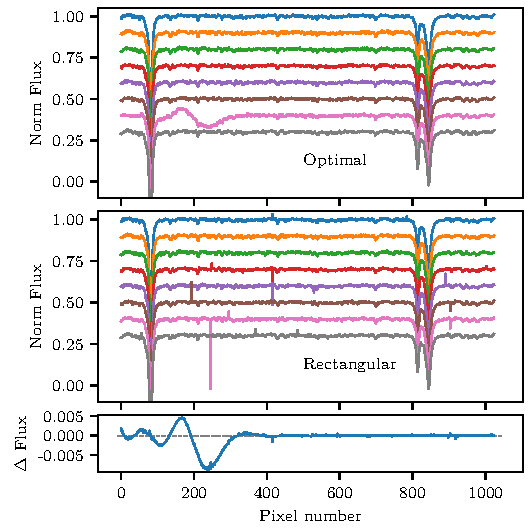
\includegraphics[width=\hsize]{images/fig1.pdf}
    \caption{Example of an artefact in the optimally extracted spectra. The top panel contains the 8 normalized nod spectra after optimal extraction, while the middle panel shows the rectangular extraction for the exact same spectra. A vertical offset is included between each spectra. A single large spike in the seventh nod (pink) near pixel 230 creates a wide and noticeable artefact in the optimal extraction. The bottom panel shows the difference between a combined spectrum using the optimal nods only and a combined spectrum in which the seventh nod is replaced with its rectangular counterpart. The nod spectra are in observation order from top to bottom.}
    \label{fig:nod_artefacts}
\end{figure}

A custom \textsc{iraf}\footnote{\textsc{Iraf} is distributed by the National Optical Astronomy Observatories, which are operated by the Association of Universities for Research in Astronomy, {Inc.}, under cooperative agreement with the National Science Foundation.}~\citep{tody_iraf_1993} reduction pipeline~\citep{figueira_radial_2010} was used to reduce the observations. It provides for automated dark and non-linearity corrections using the non-linearity coefficients provided by ESO, as well as the flagging and replacement of bad pixels. The images were corrected from sensitivity variations by dividing by the flat-field image corrected from the blaze function effect. The nodding pairs were mutually subtracted and the order tracing was fitted using either linear or cubic splines, selected for each detector.

Each spectra was extracted twice using the \emph{rectangular} and \emph{optimal} extraction algorithms.
The \emph{rectangular} extraction performs a rectangular aperture sum in the spatial direction while the \emph{optimal} extraction~\citep{horne_optimal_1986} also includes variance weighting to reduce the impact of the noise and deviant pixels on the total flux measurement. {The extracted nod-cycle spectra are normalized by dividing each by a polynomial fitted to the continuum.}

The nod-cycle spectra were averaged to create a combined spectra with a higher signal-to-noise.
Where possible the 8 optimally extracted spectra were combined, but several nod spectra were replaced with their rectangular counterparts because spectral artefacts were visually identified in the \emph{optimal} nod spectra. For the replacement nods, a iterative 4-\(\sigma\) rejection algorithm\footnote{Found at \url{https://github.com/jason-neal/nod_combination}} was applied to remove the bad pixels that were not removed in the \emph{rectangular} extraction.

An example of a large extended artefact is given in Fig.~\ref{fig:nod_artefacts}. The top and middle panels show the the 8 normalized nod spectra for the \emph{optimal} and \emph{rectangular} methods respectively. In the top panel there is a clear deviation in the seventh nod spectra around pixel 200, which corresponds to a spike in the middle panel. The bottom panel shows the difference in the combined average spectra, between using only the optimal spectra and replacing those with artefacts, in this case the seventh spectrum. These artefacts were observed to create flux deviations in the combined spectra up to \(\sim\)0.5 per cent.

Several parameters of the reduction pipeline were adjusted in an attempt to  remove these artefacts with limited success, e.g. the $\sigma$ rejection limits and the aperture width. In a small number of instances allowing the aperture width to be automatically adjusted removed the artefacts. These artefacts had not been observed with this pipeline in previous works in the \textit{H}-band, so these artefacts may have some wavelength dependence.

The continuum normalization and nod combining steps were also performed with \textsc{iraf} while the following post reduction procedures and analysis utilize \textsc{python}. This pipeline was chosen over the ESO CRIRES pipeline because it was semi-automated, seemed relatively simple to use and, initial tests appeared to contain less bad pixel/cosmic ray artefacts in the extracted spectra compared to the ESO pipeline. In hindsight, the spectral artefacts observed decreased it's ease of use.

\subsubsection{Wavelength calibration}
\label{subsec:wave_cal}
There is a known issue with the wavelength calibration from the CRIRES Th-Ar calibrations~\citep{kerber_laboratory_2009}, due to the low density of Th-Ar lines in the nIR and the alignment with the detectors narrow wavelength range (e.g.\ CRIRES-POP~\citep{nicholls_crirespop_2017}).
Therefore, we use the telluric absorption lines present in each observation as the wavelength reference. Instead of directly using the HITRAN database~\citep{rothman_hitran2012_2013} for the line positions of the telluric spectra (e.g.~\citep{brogi_signature_2012,brogi_carbon_2014,dekok_detection_2013}), we use TAPAS atmospheric transmission models~\citep{bertaux_tapas_2014} obtained for each observation. These in turn use the HITRAN database but include atmospheric profiles and physical measurements to model the telluric absorption strength.

The centroid of each telluric line is obtained by fitting the telluric transmission spectrum, \(T\), as a sum of Gaussian functions (subtracted from the continuum) representing the telluric lines,

\begin{equation}
T(\lambda) = 1 - {\Sigma}_{i}\ G(\lambda, A_{i}, {\mu}_{i}, {\sigma}_{i}),
\end{equation}

where \(G\) is a Gaussian function of the form

\begin{equation}
G(\lambda, A, \mu, \sigma) = {A \textrm{e}}^{{-(\lambda-\mu)}^{2}/2\sigma^{2}}
\end{equation}

and \(A\), \(\mu\), \(\sigma\) are the amplitude, central wavelength, and standard deviation for each line respectively. {Although telluric lines are actually Voigt profiles, they are not fully resolved in the nIR and their shape is dominated by the instrumental profile. The instrumental profile for CRIRES has been shown to be well represented by a Gaussian shape~\citep{seifahrt_synthesising_2010}.}

The observed spectra contain two different components: the stellar and telluric lines multiplied together. These were fitted with two Gaussian-sum models multiplied together, with the identification of telluric and stellar lines performed {by hand} for each spectra, using the synthetic telluric models as the reference.
\begin{align}
I_{obs}(x) &= I_{tell}(x) \times {\bl I_{star}}(x) \nonumber \\
I_{obs}(x) &= \Big(1 - {\Sigma}_{j}\ G(x, A_{j}, {\mu}_{j}, {\sigma}_{j})\Big) \times \Big(1 - {\Sigma}_{k} G(x, A_{k}, {\mu}_{k}, {\sigma}_{k})\Big), \label{eqn:obs}
\end{align}

where \(x\) is the pixel coordinate of the extracted spectra.

The wavelength solution was obtained by fitting a second order polynomial, shown to be sufficient for higher precision RV studies~\citep[e.g.][]{bean_groundbased_2010, figueira_radial_2010, seifahrt_synthesising_2010}, to the centroid values \(\{\mu(x), \mu(\lambda)\}\) obtained from the telluric component of the observed spectra and telluric model respectively.

Much like issues with Th-Ar calibrations this method only works well when there is sufficient coverage of telluric lines on the detector. For the wavelength setting of these observations, the spectra from the second detector (top right panel of Fig.~\ref{fig:detector4allspectra}) only has two large telluric lines present with several small lines, with relative depths smaller than 1 per cent, which are difficult to identify. This deteriorated the calibration stability for the second detector. With the lack of telluric contamination and stellar lines on the second detector it may have been ideal for the detection of a faint secondary spectra; unfortunately the wavelength calibration quality varies in an inverse way.

We note that there are many variations on this wavelength-calibration technique including those integrated within programs such as \textsc{TelFit}~\citet{gullikson_correcting_2014}, and ESOs \textsc{Molecfit}~\citet{smette_molecfit_2015}, that perform telluric correction and re-calibrate the wavelength axis themselves. {Including features such as concurrent fitting of a stellar spectral model, adjusted for RV, along with the telluric model could help to improve the wavelength calibration preformed here. For example~\citet{piskorz_evidence_2016} performed wavelength calibration using only a telluric line model at other nIR wavelengths but had to specifically include a stellar model around 2\,$\mu$m where the telluric lines are weaker.}

\begin{figure*}
    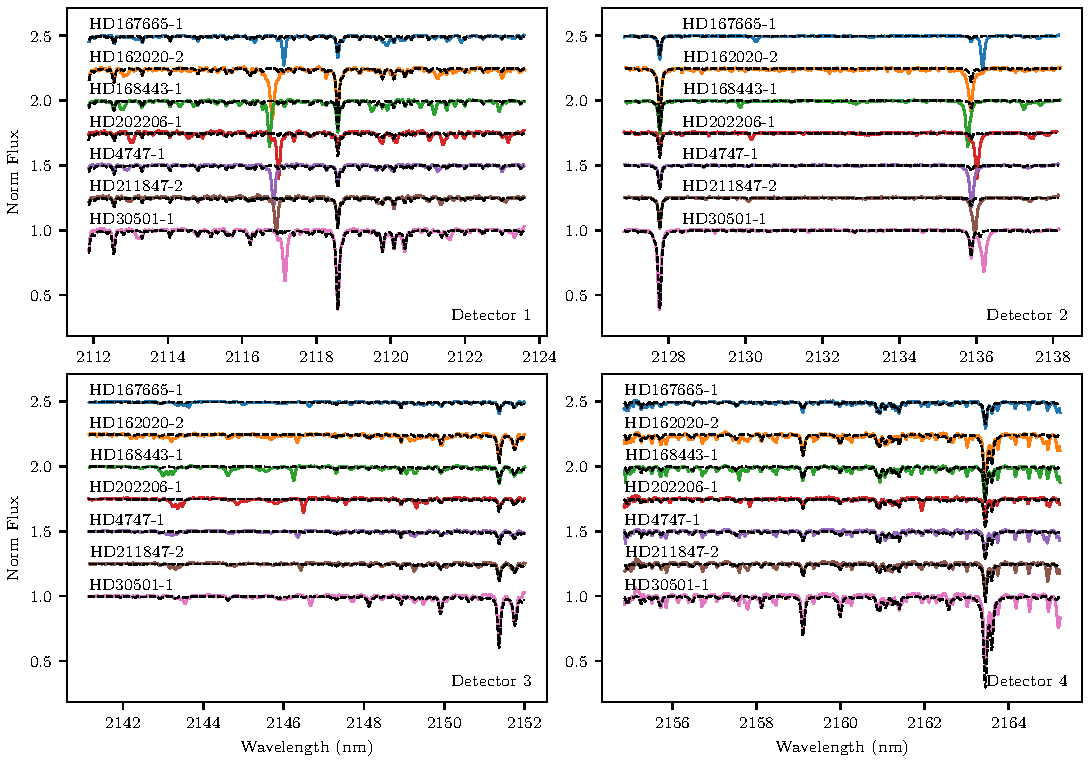
\includegraphics[width=0.8\hsize]{images/fig2.pdf}
    \caption{Extracted, normalized and wavelength calibrated spectra for a single observation of each target. The target name is given above each spectrum along with the observation number. Each panel is the spectra from a single detector 1--4 in order of increasing wavelength. The black dashed lines indicate the unique telluric spectrum used for wavelength calibration and telluric correction for each observation.}
    \label{fig:detector4allspectra}
\end{figure*}

\subsubsection{Telluric correction}
\label{subsec:telluric_correction}
Ground based observations require the removal of the absorption lines introduced by Earth's atmosphere. The observations analysed here were taken in an atmospheric window of the \textit{K}-band in order to reduce the absorption introduced by the atmosphere~\citep{barnes_hd_2008}. To correct for the remaining telluric line contamination the spectra were divided by the TAPAS\citep{bertaux_tapas_2014} atmospheric transmission models for each observation. These synthetic telluric models were used to avoid the observing overhead necessary to perform telluric standard star exposures~\citep{vacca_method_2003}, and they have been demonstrated to be superior in the quality of the correction relative to the telluric standard approach~\citep[e.g.][]{cotton_atmospheric_2014}.

Before the correction, the depth of the telluric lines were re-scaled to match the airmass of the observation using the relation \(\rm T = T^{\beta}\), where \(\rm T\) is the telluric spectrum and \(\beta\) is the airmass ratio between the observation and model. This changed the depth of most absorption lines to match the observations, but does not correctly scale the deeper \(\rm H_{2}O\) lines. The scaled telluric model is interpolated to the wavelengths of the observed spectrum and then used to correct the observed spectra through division, leaving behind a telluric corrected spectra. An example of a telluric corrected spectra is shown in the middle panel of Fig.~\ref{fig:spectral_example}, with the light blue shading indicating where the deeper telluric lines were.

We attempted the technique suggested by~\citet{bertaux_tapas_2014} to address the poor \(\rm H_{2}O\) airmass scaling, to fit a scaling factor to the \(\rm {H}_{2}O\) absorption lines before convolution to the instrument resolution. This was achieved by first dividing the spectrum by a telluric model with only non-\(\rm H_{2}O\) constituents, convolved to the observed resolution, and scaled by the airmass to remove the non-\(\rm H_{2}O\) lines. Then a model with only \(\rm H_{2}O\) lines at full resolution was scaled by a factor \(\textrm{T}^{x}\), convolved to \(\rm R=50\,000\) and compared to the observed spectra. The factor \(x\) was fitted to find the best scaling factor for the \(\rm H_{2}O\) lines.

This method corrected the deeper telluric lines well for a few spectra in our sample, but in many cases we found that the fitted scaling factor was affected by the presence of blended stellar lines (attempting to fit those also). It was also strongly influenced by the deepest \(H_{2}O\) telluric lines in the spectra analysed. We find that the telluric correction of the deep \(\rm H_{2}O\) lines could be improved with this technique, but, at the cost of worsening the correction of the many smaller \(\rm H_{2}O\) lines. Since the smaller \(\rm H_{2}O\) lines covered more of the spectrum in this region than the larger lines we chose not to continue with this separate \(\rm H_{2}O\) scaling. One possible solution for this would be to perform a piece-wise telluric correction, performing this step only for the deeper \( \rm H_{2}O\) lines, or by using one of the other tools that fits the telluric model to the observations. This technique could also benefit from a larger wavelength span that would enable blended lines to be ignored while having sufficient deep \(\rm H_{2}O\) lines to fit the scaling factor correctly. This small experiment shows that a simple scaling is not enough to correct for the absorption in an effective way, for this case.

After the telluric correction is performed, the spectra are corrected for Earth's barycentric RV using the \textsc{helcor} \textsc{PyAstronomy}\footnote{https://pyastronomy.readthedocs.io} function ported from the \textsc{reduce idl} package (See~\citet[][]{piskunov_new_2002}).

\subsection{Tapas models}
\label{subsec:tapas_models}
We used telluric line models to wavelength calibrate the reduced spectra in Sect.~\ref{subsec:wave_cal} and to correct for the atmospheric absorption in Sect.~\ref{subsec:telluric_correction}. We utilized the TAPAS (Transmissions of the AtmosPhere for AStronomical data) web-service\footnote{\url{http://www.pole-ether.fr/tapas/}}~\citep{bertaux_tapas_2014} to obtain atmospheric transmission models for each observation. TAPAS uses the standard line-by-line radiation transfer model code LBLRTM~\citep{clough_linebyline_1995} along with the 2008 HITRAN spectroscopic database~\citep{rothman_hitran_2009} and Arletty atmospheric profiles derived using meteorological measurements from the ETHER data centre\footnote{\url{http://www.pole-ether.fr}}, which has a 6 hour resolution in atmospheric profiles.
We use the mid-observation time to retrieve transmission models for each observation, with the Arletty atmospheric profiles\footnote{Nearest of the 6 hourly profiles} and vacuum wavelengths. The telluric models were retrieved without any barycentric correction to keep the telluric lines at a RV of zero with respect to the instrument. We obtained one model with all provided species present, convolved to a resolution of \(\rm R=50\,000\), and another two models without an instrumental profile convolution applied. For these two extra models, one contained only the transmission spectra of \(\rm H_{2}O\) while the other was for all other constituents except \(\rm H_{2}O\). This was to explore a known issue~\citep{bertaux_tapas_2014} with the depth of \(\rm H_{2}O\) absorption lines in Sect.~\ref{subsec:telluric_correction}.

\subsection{Wavelength masking}
Several wavelength masks are applied to remove wavelength regions from which we cannot extract spectral information.
Firstly, regions near the edges of each detector where the wavelength solution is extrapolated outside of the calibrating telluric lines were removed, reducing the effective size of each detector by about \(10\) per cent or \(\sim\)100~pixels.

Secondly, any remaining artefacts present in the spectra were masked out and the centres of deep telluric lines where telluric correction was not corrected properly. These sometimes resulted in ``emission-like'' peaks in the corrected spectrum. These two factors resulted in masking out around a further 10 per cent of the observed spectra.

In Sect.~\ref{sec:results} a further wavelength restriction is used to mask out regions where there is a large mismatch between the observed spectrum and the closest synthetic spectra for the host star. This significantly restricts the wavelength span utilized to around only 43 per cent. The masked regions are shown as the shaded areas in Fig.~\ref{fig:visualinspection-hd2118471}.


\section{Binary synthetic spectral recovery}
\label{subsec:companion_recovery}
We explore spectral fitting the observations with a binary model with the aim to detect the presence of the faint spectra which is in combination with the host star. The observed spectra are fitted with a binary combination of two synthetic spectral models, using \(\chi^{2}\) methods which have been extensively used in the literature~\citep[e.g.][]{astudillo-defru_harps_2015, passegger_fundamental_2016, zechmeister_spectrum_2018,nemravova_xtauri_2016}. {The parameters of the synthetic spectra fitted to the companion should provide an indication of the properties of the companion.}

\subsection{Synthetic PHOENIX-ACES models}
\label{subsec:spec_models}
The PHOENIX-ACES synthetic spectra library~\citep{husser_new_2013} is used as the reference spectra to compose binary models for the spectral comparison. It uses the most recent version (16) of the PHOENIX code and is suitable for the spectra of cool stars. The full parameter space of the PHOENIX-ACES spectra is given in Table~\ref{tab:phoenix} but we restrict our usage to the domain covered by the observation targets.

%!TEX root = ../nir_companions.tex

\begin{table}
    \centering
    \caption{Full parameter space of the PHOENIX-ACES spectral grid.}
    \begin{tabular}{lr@{ -- }lc}  % Seperate columns with --
        \toprule
        & \multicolumn{2}{c}{Range}       & Step size\\
        \midrule
        \ \(T_{\textrm{eff}}\) [K] &  2300 & 7000  & 100 \\
        &  7000 & 12000 & 200 \\
        \  logg     &  0.0 & +6.0   & 0.5 \\
        \ [Fe/H]   &  -4.0 & $-$2.0  & 1.0 \\
        &  -2.0 & +1.0  & 0.5 \\
        \  \(\alpha\)/Fe &  -0.2 & +1.2  & 0.2 \\
        \bottomrule
    \end{tabular} \label{tab:phoenix}
\end{table}


The spectral model libraries were accessed using the useful ``grid tools'' interface provided in the \textsc{Starfish}\footnote{\url{https://github.com/iancze/Starfish}} \textsc{python} package~\citep{czekala_constructing_2015}, which made it efficient to load in the spectra when needed.

The synthetic spectra are multiplied their wavelength to convert them into photon counts, ignoring multiplicative constants, as done in~\citet{figueira_radial_2016}\footnote{Synthetic models provide the spectral energy distribution (\(\rm erg\,s^{-1}\,cm^{2}\,cm^{-1}\)).}. The spectra are also convolved with a Gaussian kernel to match the resolution of the observations (\(\rm R=50\,000\)). Due to the distributive property of convolution it is efficient to apply convolution once to each synthetic spectra first, before the spectral pairs are combined.

The PHOENIX-ACES models include dust in equilibrium with the gas phase while ignoring dust opacity and does not include any mixing/settling which is important for cooler BD atmospheres. They set a minimum library \(T_{\textrm{eff}}=2300\)~K to avoid the temperatures at which the modelling of clouds is necessary. This unfortunately limits the use of this library for this technique to the largest mass companions in our sample. For example a \(T_{\textrm{eff}}=2300\)~K corresponds to a BD with \(\rm M\sim84~M_{Jup}\) at 5 Gyr from the~\citet{baraffe_evolutionary_2003} evolutionary models.

There are other spectral models that extend below 2300~K such as the {BT-Settl} models\citep{allard_btsettl_2013,baraffe_new_2015}. These are discussed in Sect.~\ref{subsubsec:BT-Settl}.

\subsection{\texorpdfstring{\(\chi^{2}\)}\ \ method}
\label{subsec:chi2}
The well known \(\chi^{2}\) technique measures the weighted sum of the squared deviation between the observation (\({O}_{i}\)) and the computed models (\(C_{i}\)), with the minimum \(\chi^2\) value representing the best-fit parameters. The \(\chi^{2}\) is defined as
\begin{equation}
\chi^{2} = {\Sigma}_i { (O_{i} - C_{i})}^2 / {\bl {\sigma}_{i}^{2}}\,,
\end{equation}
  where \({\sigma}_{i}\) is the error on each measurement. We estimate the \(\sigma\) of each spectrum using the \(\beta\sigma\) method~\citep{czesla_posteriori_2018}, using the MAD (median absolute deviation about the median) robust estimator. {This method estimates the spectral noise using numerical derivatives of the spectra. We followed the procedure outlined in~\citet{czesla_posteriori_2018}, analysing the results from successive parameter combinations to settle on an order of approximation (derivative level) of 5, and a jump parameter (pixels skipped to avoid correlations) of 2.} We apply the same \(\sigma\) value to all points \({\sigma}_{i} = \sigma\). The \(\beta\sigma\) method provided \(\sigma\) estimates for the target spectra which correspond inversely to signal-to-noise ratios between 100--500. These values are similar to the those given in Table~\ref{tab:observations} which were calculated from the continuum of detector 2 only.

The computed models are described in Sect.~\ref{models} and their output is interpolated to the wavelength grid of the observed spectra. The \(\chi^{2}\) is calculated by comparing the model and observation at each point. The results from all computed models is a multidimensional grid of \(\chi^2\) values for each combination of parameters, namely the spectral temperature, host RV, and companion RV for each detector, observation and target.

We obtain the global minimum of the multidimensional \(\chi^{2}\)-space to represent the best fit to the observed spectra. We sum the multidimensional \(\chi^{2}\) across multiple detectors and determine a global minimum \(\chi^{2}\) for the whole observation \(\chi^{2}_{obs} = \Sigma^{N}_{n=1} \chi^{2}_n\), where \(N\) is the number of detectors used. We do not, however, combine the \(\chi^{2}\) values across the separate observations as the RV parameters of the host and companion will vary between each observation.

The inverse survival function of the \(\chi^2\) distribution is used to determine the confidence levels on the minimum \(\chi^2\) parameters. The inverse survival function returns a \(\Delta\chi^2\) value from the minimum \(\chi^2\) value for a given sigma level and degree of freedom\footnote{In \textsc{python} with the \textsc{scipy} package this is a single line \texttt{scipy.stats.chi2(dof).isf(1-p)}, where \(p = 0.68\) for 1-\(\sigma\), and dof is the degree of freedom.}.
For example, the \(\Delta \chi^2\) for a single degree of freedom required for the 1-, 2-, and 3-\(\sigma\) levels is 1, 4, and 9 respectively~\citep{bevington_data_2003}. This method assumes that the measured flux is observed with a SNR sufficiently high so that the noise on the spectrum is approximately Gaussian, and the \(\chi^2\) method appropriate.

For a given observation, the \(\chi^{2}_{red}\) is computed by \(\chi^2_{red} = \chi^2 / \nu\) where \(\nu = n - m\), the number of observed pixels, \(n\), minus the number of parameters of interest, \(m\)\footnote{\(m=2\) or 4 in the examples explored below}, and is performed after the summation over the detectors.

\subsection{Computed model spectra}
\label{models}
\subsubsection{Single component model}
\label{subsubsec:single-model}
The single component model \(C^{1}_{i}\) comprises of a single synthetic spectrum, \(J\), (with model parameters \(T_{\textrm{eff}}\), logg, [Fe/H], [\(\alpha\)/Fe]) and is Doppler shifted by a RV value \({rv}_1\).

It can be summarized by the equation, 
\begin{equation}
\rm C^{1}_{i}(\lambda) = J(\lambda_0(1-\frac{{rv}_1}{c})),
\end{equation}

where \(\lambda\) is the shifted wavelength, \(\lambda_0\), the model rest wavelength and, \(c\), the speed of light in a vacuum. The model's flux is then continuum normalized to unity to match the observed spectra, and interpolated to the wavelength grid of the observation.

This single component model is similar to the \(\chi^2\) fitting performed by \citet{passegger_fundamental_2016}. We apply the same re-normalization (see Sect.~\ref{subsec:renorm}) to account for slight differences in the continuum level and possible linear trends between the normalized observation and model. Unlike \citet{passegger_fundamental_2016} we do not apply any dynamical masking to sensitive lines to make the the \(\chi^2\) minima more distinct or linearly interpolate the stellar parameters between the grid models to obtain high precision stellar parameters. This is due to the differnces in our end goals, detecting a secondary spectral component, compared to deriving precise stellar parameters. We also include radial velocity components to the \(\chi^2\) fitting, which is not included in~\citet{passegger_fundamental_2016}.

\subsubsection{Binary model}
\label{subsubsec:binary-model}
In the binary situation we consider the superposition of two synthetic spectral components, one each for the host and companion respectively. Both spectra are Doppler shifted by \({rv}_1\) which represents the RV motion of the host star, while the companion spectra is also Doppler shifted by a second RV, \({rv}_2\), representing the RV offset between the host and companion. In this way the mean motion of the system relative to Earth is captured only in \({rv}_1\). The two spectra are scaled by their squared radius (see Sect.~\ref{subsection-radius}) and then added together, thus fixing their relative amplitude.
Given two spectral components \(J_{1}\) and \(J_{2}\) with radii \(R_1, R_2\) this equates to
\begin{align}
\rm C^{2}_{i}(\lambda) = &  J_{1}(\lambda_{0}(1 - \frac{rv_{1}}{c}))\times R_{1}^2 +\nonumber \\
& J_{2}(\lambda_{0}(1-\frac{rv_{1}}{c})(1-\frac{rv_{2}}{c}))\times R_{2}^2
\end{align}

The continuum of the combined spectrum is fitted with an exponential and then normalized by dividing it by the fitted result as we assume we are in the Rayleigh-Jeans regime. This assumption is wavelength dependent and other appropriate continuum normalization techniques are also valid. In the case of a BD companion around an FGK star investigated here, the continuum is dominated by the contribution from the host star as it contributes the majority of the spectrum with flux ratios around 2110--2160~nm below \(\sim\)1 per cent.

We combine the models in this way to represent the correct absolute flux ratio of the components. The median flux ratio between the two components is calculated for the wavelength range used here as an indication of the flux ratio level.

The binary model should provide meaningful information about the companion parameters (e.g.\ \(T_{\textrm{eff}}\)) and a estimate of the flux ratio of the system. These can be combined with the~\citet{baraffe_evolutionary_2003} models to constrain the mass of the companion. However, we need to be careful with this model as the inclusion of extra spectral components and associated parameters could also provide a better fit to observations which do not have a companion, by fitting components of the noise.\\

{The full list of grid parameters for the binary model are \(T_{\textrm{eff}}1\),  \(\rm logg_1\), [Fe/H]$_1$, [\(\alpha\)/Fe]$_1$, ${rv}_1$, \(T_{\textrm{eff}}2\), \(\rm logg_2\), [Fe/H]$_2$, [\(\alpha\)/Fe]$_2$, ${rv}_2$ where the subscripts 1 and 2 indicate the host and companion models respectively.}

\subsubsection{Effective radius}
\label{subsection-radius}
To combine the two synthetic spectra with the correct observed flux ratio we need to integrate the emitted flux over the effective surface area of each emitting body respectively. Ignoring the common multiplicative constants that will disappear with normalization, we scale the two synthetic spectra individually by the square of their respective radii, \(R_1\) and \(R_2\).

In this work we use the effective radius (PHXREFF keyword) of each component from the PHOENIX model headers. This is the radius used in modelling of the stellar atmospheres. We use this radii as it is directly tied to each model spectrum, and already available. The ratio of the radii from the two synthetic spectra in the binary models are provided in Table~\ref{tab:example_params}.

We are aware that using these radii has its limitations, since as stated previously, there is a degeneracy in BD mass, age, and luminosity of the companion, and in particular a combination of radius-mass and radius-age relationships~\citep{sorahana_radii_2013}. Using the PHOENIX-ACES model effective radius does not allow for any independent age constraints to be incorporated, or allow for any variability in the radii to account for uncertainties.

The targets analysed here do not have transits, but if the radius ratio can be independently determined from the photometric transit method~\citep{deeg_photometric_1998} then this could be used to constrain the radius ratio used when combing the binary model spectra instead.

\subsection{Re-normalization}
\label{subsec:renorm}
Slight trends in the continuum level between the observed spectra and computed models were removed using the re-normalization following~\citep{passegger_fundamental_2016}:
\begin{equation}
F^{obs}_{re-norm} = F^{obs} \cdot \frac{\textrm{continuum fit}_{model}}{\textrm{continuum fit}_{observations}}.
\end{equation}
The polynomial continuum fits to the normalized observations and models are used to re-normalize the observed spectrum to the continuum of the models. For detectors 1--3 a polynomial of first degree was used, while for detector 4 a quadratic is needed to fit the edge of a strong Hydrogen line (Brackett-\(\gamma\)) at 2166~nm, which lies just off of detector 4. This broad line is only observed in the synthetic spectra and not in the reduced observations. It is assumed that this was normalized out during the reduction process.

For each model we further allow the continuum level to be {\bl scaled between 0.95 and 1.05 as a free parameter} taking the model with the smallest \(\chi^2\) value.

\subsection{Reducing parameters}
\label{subsec:reduce-params}
The high dimensionality of the binary model makes it computationally challenging and difficult to analyse the \(\chi^2\) space.
For reference, the multiplicative parameter space is squared when increasing from one spectral component in the single model to a binary model, and becomes computationally expensive. In general the number of possible parameter combinations for \(c\) spectral components each with a grid of \(m\) models increases to \(c^m\). If the full set of PHOENIX-ACES library spectra (66456) is explored with a binary fit then this naively balloons to over 4.4 billion possible combinations. Half of these are not unique as the host and companion components are swapped. This is the worst case scenario and we implement a number of assumptions to vastly reduce the parameter-space enabling faster computation.

Our first assumption is to restrict ourselves to models with an Alpha element abundance ([\(\alpha\)/Fe]) of zero. This is likely a very good approximation as all our targets have solar metallicity and are thus very likely to belong to the thin disk of the Galaxy, where [\(\alpha\)/Fe] values are close to zero (i.e., solar) -- e.g.~\citet{adibekyan_chemical_2012}. Our second assumption is that the search space can be significantly reduced using the literature values for the host star given in Table~\ref{tab:starparams}. The metallicity of both components and the logg of the host star is fixed to the grid points closest to the literature values. The uncertainties on the literature measurements for metallicity (\(\sim\)0.05) and logg (\(\sim\)0.1) are both smaller than the grid steps of 0.5 for these parameters.
For the logg of the companion the~\citet{baraffe_evolutionary_2003,baraffe_new_2015} evolutionary model value are used for the given companions \(\textrm{M}_2\)/\(\textrm{M}_2\sin{i}\) and hosts age.

We use the estimated companion temperatures from the Baraffe evolutionary models given the companion \(\rm M_2\) or \(\textrm{M}_2\sin{i}\) and stellar age as a starting point for the companion spectra grid computation and extend the grid typically by \pm\(500-1000\)~K in each direction, within the model limits based on trail and error. For example we show the companion temperature grid spanning \(-600\) to \(+400\)~K in Fig.~\ref{fig:Mdwarf_contours} and \(\pm400\)~K in Figs.~\ref{fig:HD211847_simulated_contours} and~\ref{fig:HD211847_result_contours}.

The large numbers stated above also do not include the RV grid for each component. The RV grid is user defined and the number of spectra /models to consider increases when the RV grid step size is decreased (finer RV resolution). We can reduce the RV grid space significantly by tailoring it to the target being examined. For each target, we use the estimated RV values from the observation time and orbital parameters, given in Table~\ref{tab:observations} as a centre starting point for the \({rv}_1\) and \({rv}_2\) values and increment the RV within a few FWHM around those values, or out to the targets \(\rm K_1\) and estimated \(\rm K_2\) values.

The RV grid step results were explored manually but an iterative process could be implemented to refine the RV grids, starting at a larger grid with lower RV resolution then performing a higher resolution grid about the minimum \(\chi^2\) RV values. One could imagine that a good starting RV grid step size be governed by the spectral resolution, e.g.\ comparable to the FWHM velocity.

For the companions targets with fully resolved orbits the known RV of the host star, \({rv}_1\) could also have been fixed. IT However it was left free to see if the known value would be recovered by the fitting.

These very restrictive parameter selection are also the result of the poor spectral match to these observations, discussed in Sect.~\ref{subsubsec:mismatch}. Including fitting in logg or [Fe/H] lead to results of those parameters furthest from the literature value. Applying this technique in different spectral range with better spectral content may be able to include these dimensions.

\section{Results}
\label{sec:results}

%!TEX root = ../nir_companions.tex

\begin{table*}
    \centering
    \begin{threeparttable}
        \caption{Input and recovered parameters on simulations and an observation when applying a single (\(\rm C^1\)) and binary (\(\rm C^2\)) models. The logg and metallicity were fixed at \(\rm logg_1=4.50\), \(\rm logg_2=5.0\) and [Fe/H]=0.0 equally for both components. Gaussian noise was added to both simulations with a SNR of 150. {Here $m$ and $n$ are the number of data points and parameters used in each model.}}
        \begin{tabular}{c | *3c | *3c | *3c}
            \toprule
            & \multicolumn{3}{c|}{Simulation 1} & \multicolumn{3}{c|}{Simulation 2} & \multicolumn{3}{c}{Observed {HD 211847}} \\
            \midrule
            & Input & \multicolumn{2}{c|}{Recovered} & Input & \multicolumn{2}{c|}{Recovered} & Expected & \multicolumn{2}{c}{Recovered} \\
            & & \(C^1\) & \(C^2\) & & \(C^1\) & \(C^2\) & & \(C^1\)  & \(C^2\) \\
            \midrule
            \(T_{\textrm{eff}_1}\) & 5800 & 5800 & 5800 & 5700 & 5800 & 5700 & \(5715 \pm 24\) & 5900 & 5800\\
            \(T_{\textrm{eff}_2}\) & 4000 & -- & 3800 & 3200 & -- & 3100 & \(\sim\)3200 & -- & >3800\tnote{a}\\
            \({rv}_1\) & 0 & 0.1 & 0 & 6.6 & 6.6 & 6.6 & \(6.6 \pm 0.3\) & 7& 7.6 \\
            \({rv}_2\) &  10 & -- & 9.8 & 0.5 & -- &  -1& \(0.5 \pm 2\) & -- &-12.6\\
            \midrule
            \(R_1/R_2\)& 2.57 & -- & 2.71& 3.16 & - & 3.27 & 3.16 & -- & <2.71\tnote{a}\\
            \(\rm F_2/F_1\)& 0.084 & -- & 0.066 & 0.030 & -- & 0.026 & 0.030 & -- & >0.066\tnote{a}\\
            {$m$} & - & 3072 & 3072 & -- & 3072 & 3072 & -- & 2612 & 2612\\
            {$n$} & - & 2 & 4 & -- & 2 & 4 & -- & 2 & 4\\
            \(\chi^2\)& -- & 4978 & 3792 & -- & 3746 & 3630  & -- & 37688 & 33860\\
            \(\chi^2_{red}\) & -- & 1.62 & 1.24 & -- & 1.22 & 1.18 & -- & 21.3 & 19.2\\
            {BIC} & -- & -20145 & -22315 & -- & -21477& -21377& -- & 18281 & 14468\\
            \bottomrule
        \end{tabular}\label{tab:example_params}
        \begin{tablenotes}
           \item [a] {At the arbitrary upper limit for companion temperature grid (3800~K).}
        \end{tablenotes}
    \end{threeparttable}
\end{table*}


\begin{figure*}
    \centering
    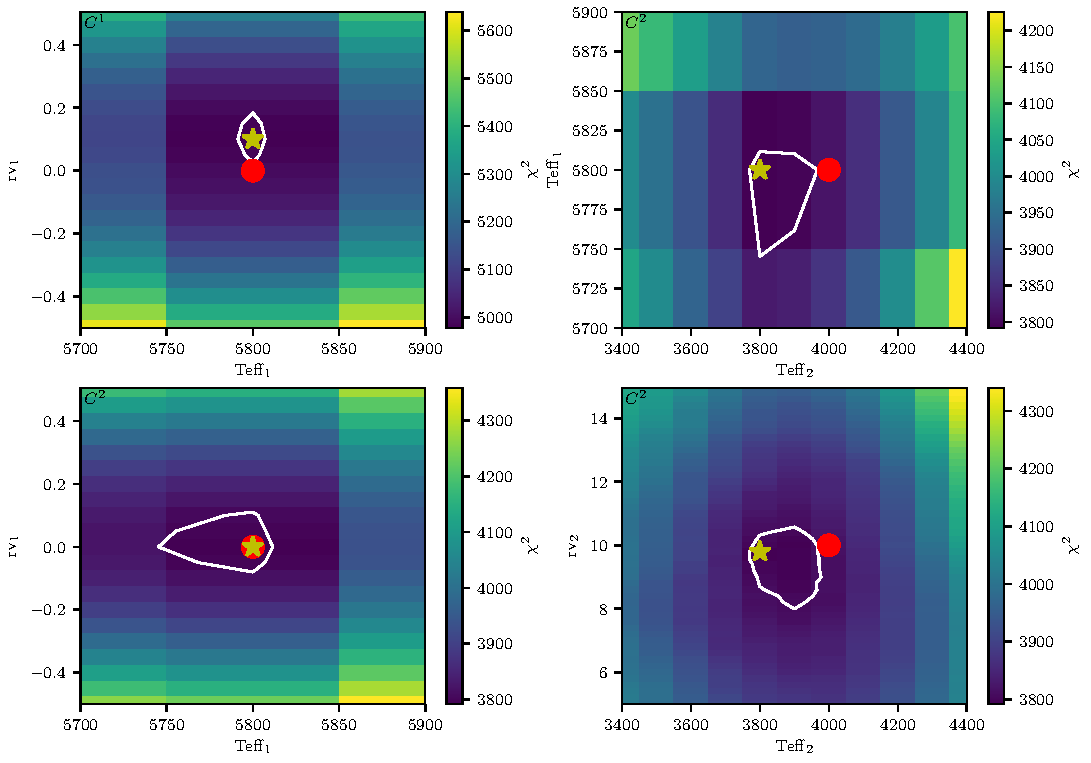
\includegraphics[width=0.8\hsize]{images/fig3.pdf}

    \caption{\(\chi^2\) results for companion recovery of a simulated binary observation of a Sun-like star (\(T_{\textrm{eff}_1}=5800\)~K) with an M-dwarf companion (\(T_{\textrm{eff}_2}=4000\)~K). The top right plot shows the application of a single component model (\(C^1\)) while the other three are using a binary model (\(C^2\)). Both left hand panels show the distribution of host temperature and host RV.\@ The top right panel shows the distribution for host and companion temperature, and the bottom right the companion temperature and radial velocity.
    The red circle and yellow star indicate the location of the simulation input and recovered parameters respectively.
    The white line shows a 3-\(\sigma\) confidence level about the minimum \(\chi^2\) solution grid point. Each box is centred on the parameter values and shows the grid resolution.}
    \label{fig:Mdwarf_contours}
\end{figure*}


\begin{figure*}
    \centering
    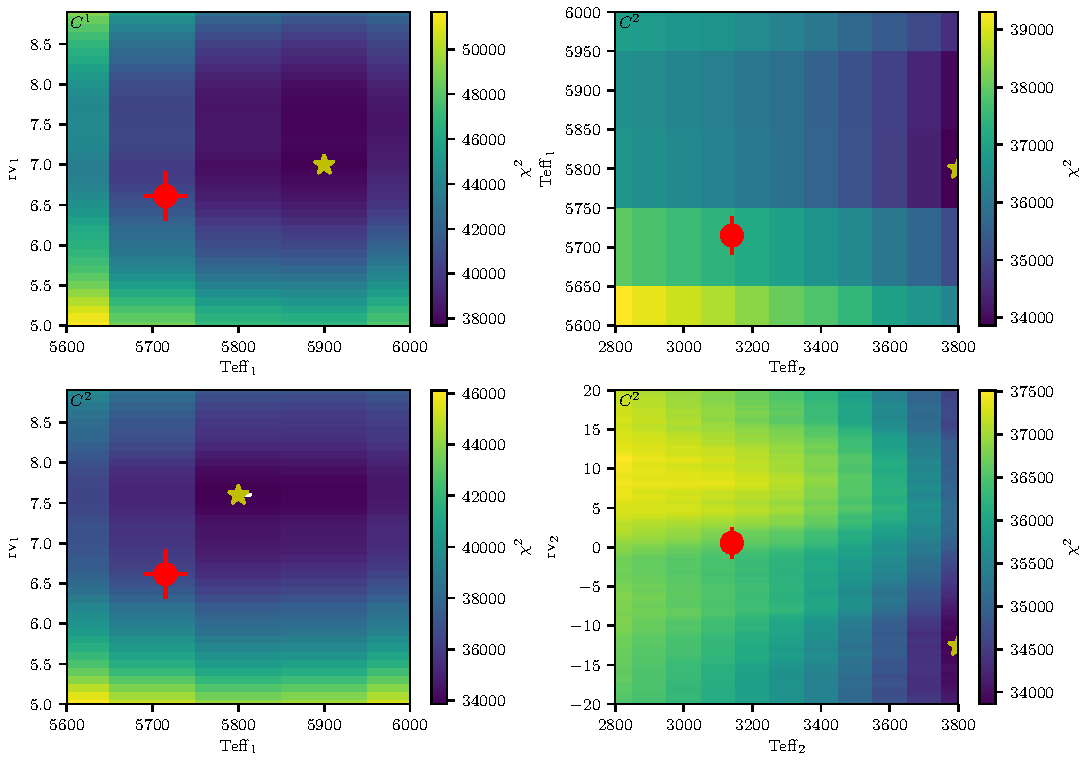
\includegraphics[width=0.8\hsize]{images/fig4.pdf}
    \caption{Similar to Fig.~\ref{fig:Mdwarf_contours}, \(\chi^2\) results for companion recovery of a simulated binary observation similar to {HD 211847}, (\(T_{\textrm{eff}_1} = 5800\)~K, \(T_{\textrm{eff}_2}=3200\)~K). The top right plot shows the application of a single component model (\(C^1\)) while the other three are using a binary model (\(C^2\)). Both left hand panels show the distribution of host temperature and host RV.\@ The top right panel shows the distribution for host and companion temperature, and the bottom right the companion temperature and radial velocity.
    The red circle and yellow star indicate the location of the simulation input and recovered parameters respectively.
    The white line shows a 3-\(\sigma\) confidence level about the minimum \(\chi^2\) solution grid point. Each box is centred on the parameter values and shows the grid resolution.}
    \label{fig:HD211847_simulated_contours}
\end{figure*}
Here we show the results from applying the companion recovery model to simulated observations and to an observation.

\subsection{Simulated binaries}
\label{subsec:simulated_binaries}
To test the companion recovery method we create simulated binary observations using PHOENIX-ACES spectra. White noise was added with a standard deviation \(\rm \sigma = 1/SNR\), for a given signal-to-noise (SNR) level. We then applied the grid-matching recovery technique detailed above and compared the resulting parameters to the inputs.

The results of two example binary simulations are displayed in Figs.~\ref{fig:Mdwarf_contours} and~\ref{fig:HD211847_simulated_contours}, both simulated with a SNR of 150. The input and recovered parameters for the binary components are indicated by the red circles and yellow stars respectively, and are given in Table~\ref{tab:example_params}.
The 3-\(\sigma\) contour is shown in white on the plots to indicate the shape of the confidence level only. The 1-\(\sigma\) contours are not shown here as they are much smaller than the temperature grid step and are not easy to visualize at this scale as they are often smaller than the marker shown at the minimum location. Each coloured rectangle is centred on the grid point, with its shape indicating the resolution of the grid space searched.

The first simulation shown in Fig.~\ref{fig:Mdwarf_contours} is for a Sun-like star with a M-dwarf companion, with a \(T_{\textrm{eff}_2} =4000\)~K. The top-left panel shows the recovered host parameters when the single model is applied to the simulated binary. The top-right and both bottom panels are the parameters recovered when using the binary model. Both left-hand panels display the parameters for the host component to easily compare between models. With both models the host temperature \(T_{\textrm{eff}_1}\) is correctly recovered. The host RV, \({rv}_1\), is 0.1\kmps{} (two grid spaces) different from the simulated value for the single component model and is correctly recovered with the binary model.

The minimum \(\chi^2\) location for the companion temperature is 200~K below the simulated value, and the RV of the companion recovered is 0.2\kmps{} below the input value. The input values for the companion are just outside of the 3-\(\sigma\) contours shown. The flux ratio for the input is 0.08 while the flux ratio recovered is 0.066.

The second simulation shown in Fig.~\ref{fig:HD211847_simulated_contours} is performed with parameters to mimic the observation of our target with highest flux ratio, {HD 211847}. In this simulation the single component model recovers a host with the correct RV but a temperature 100~K higher than the input value. Again, adding the companion with the binary model recovers the correct host temperature. The companion temperature recovered is 100~K lower than the input temperature and the RV is different by 2\kmps{} which is around one third the FWHM.

In this case with a companion RV offset, \({rv}_2\), near 0\kmps{} the host and companion lines are blended. The same spectral lines from both components are trying to match to the same features of the spectra, making it more difficult to recover the companion parameters. In the bottom right panel there appears to be multiple minima for different \({rv}_2\) and \(T_{\textrm{eff}_2}\) combinations, which we assume is partially due to the small \({rv}_2\).

In both simulations the reduced \(\chi^2_{red}\) for the binary model is closer to 1. This is not surprising as the binary model contains extra parameters. As mentioned above, we need to be careful, as the extra components from the binary may just happen to fit components of the noise when a binary is not present, or in our case has a low flux ratio.
{We {\bl analyze} the significance between the two models using the ``Bayesian Information Criterion''(BIC)~\citep{schwarz_estimating_1978}; }
\begin{equation}
BIC = n\ln{(m)} - 2\ln{(\hat{L})}.
\end{equation}
{Here $n$ and $m$ are the number of parameters and data points respectively and \(\hat{L}\) is the maximum of the Gaussian {\bl likelihood} function }
 \begin{equation}
 \hat{L} = \left(\frac{1}{\sigma \sqrt{2\pi}}\right)^m \exp{\left(-\frac{\chi^2}{2}\right)},
 \end{equation}
 {written in terms of \(\chi^2\) and a fixed $\sigma$ for all data points. The maximum {\bl likelihood} of a Gaussian distribution is equivalent to minimizing the \(\chi^2\). In both simulations \(\Delta BIC >10\) so the preference of the binary model, with the lower BIC value, over the single component model is considered \emph{significant}.}

\subsection{HD211847 observation}
\label{subsection:results-hd211847}
{HD 211847} is the best candidate for detection as it has a \(\rm 155~M_J\) low-mass star companion~\citet{moutou_eccentricity_2017}. The angular separation of the two bodies is 222 mas (or 11.3 au). Even though it is not a BD it has the highest estimated flux ratio in our sample, of 0.03 based on the~\citet{baraffe_new_2015} evolution models and the known companion mass (see. Table~\ref{tab:estimatedparameters}). The angular separation of HD211847B is 222 mas with a projected distance of The result of applying \(\chi^2\) fitting to the second observation of {HD 211847} is shown in Fig.~\ref{fig:HD211847_result_contours}.

For this target the metallicity of both components was fixed to 0.0 and the logg for the host was fixed at 4.5. The logg for the companion is fixed to 5.0, based on the~\citet{baraffe_new_2015} evolutionary models for the given companion mass and system age. The orbital solution was used to refine the RV search space of both components. The span RV for the companion was extended until a value inside the RV bounds was found.

Again the top left panel of Fig.~\ref{fig:HD211847_result_contours} shows the recovery with a single component model with the other three for the binary model. The single component model finds a temperature of 5900~K for the host with a \({rv}_1\) of 7\kmps{}. This is 200~K and 0.4\kmps{} different above the expected parameters. The binary model finds a host temperature of 5800~K, which is the second closest model to the literature value, >100~K different. The host RV value recovered with the binary model is 7.6\kmps{}, which is 1\kmps{} higher than expected.  For the single component model there is a barely noticeable secondary minima near this 7.6\kmps{} RV value recovered by the binary model. Again these RV differences are smaller than the FWHM of the lines. The 3-\(\sigma\) contour is small, just visible on the right hand side of the star in the bottom left panel, and hidden behind the markers in the other panels.


For the companion in the binary model, on the right side of Fig.~\ref{fig:HD211847_result_contours}, the minimum \(\chi^2\) for the companion temperature is at the upper temperature limit of the grid shown. If we extend the grid of companion temperature towards higher temperatures the best fit location continues to increase in temperature, continually hitting the upper limit until it is close to the host temperature, >2000~K above the expected companion temperature. When the companion temperature becomes this high it also affects the recovered parameters for the host star to offset the features of the brighter companion.

The \(\chi^2_{red}\) values for the single and binary models are 21 and 19 respectively, far from 1, indicating that both models are a poor fit to the observations. {The $\Delta BIC = 3812 >10$ indicating that binary model is still preferred.} We plot the binary model for the best fit solution alongside the observed spectra in Fig.~\ref{fig:visualinspection-hd2118471}. We see that there is a large spectral mismatch between the synthetic models and the observation. Extra wavelength masking was applied to many of the largest mismatched synthetic lines to remove their influence. The grey areas mark regions which have been masked out, either from the centres of deep telluric lines (the thin masks matching spectral gaps), or the more prominent mismatched lines in the synthetic spectrum excluded from the \(\chi^2\) analysis. One clear example of a mismatched line is a synthetic line at 2132.5~nm that is clearly not observed in detector 2 (top right). Even with the majority of the mismatched lines removed the detection of the companion was still unsuccessful.

For detectors 1 and 2 it appears that the synthetic spectra contain many more deeper lines than observed. For detector 3 the red half of the detector was masked out as there appears to be an offset between the observed lines. With 3--4 lines that appear to be consistently offset from the observation it could be a wavelength calibration issue, although the telluric lines appear to be sufficiently corrected in this region, attesting for the quality of the wavelength calibration, and making it incompatible with the offset. For detector 4 the observed lines do not agree at all with the models. With many observed lines not in the model and only one line with some agreement in wavelength, detector 4 is masked out completely and not used in the \(\chi^2\) fit. Individual inspection of the \(\chi^2\) results for each detector also revealed that there was a large discrepancy between the 4th detector and the other three, with a different RV value for the host star and a \(\chi^2\) values an order of magnitude higher. The edge of a deep Hydrogen line (Brackett-\(\gamma\)) off the edge of the detector 4 is also clearly seen in the continuum of the model >2162~nm.

We applied this same method to the remaining targets, with similar results. In brief, we conclude that the companion spectra cannot be correctly detected in our data using this method.

\begin{figure*}
    \centering
    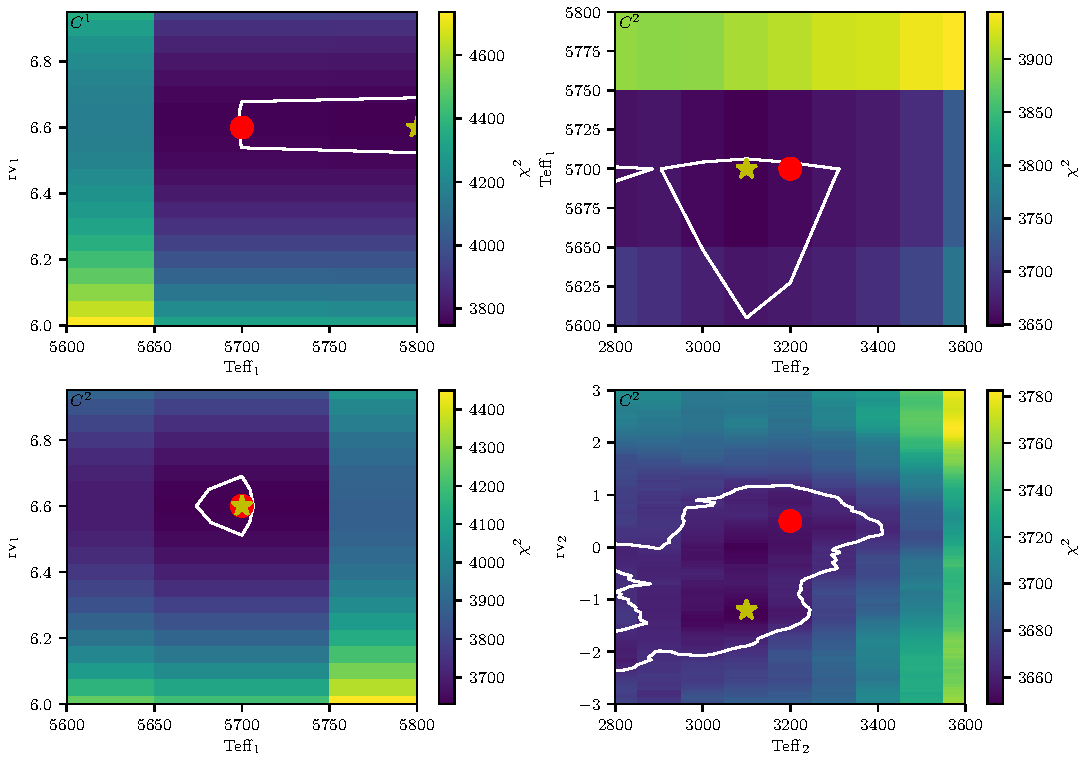
\includegraphics[width=0.8\hsize]{images/fig5.pdf}
    \caption{\(\chi^2\) result grid for observation 2 of {HD 211847}, similar to Figs.~\ref{fig:Mdwarf_contours} and~\ref{fig:HD211847_simulated_contours}. The top right plot shows the application of a single component model (\(C^1\)) while the other three are using a binary model (\(C^2\)). Both left hand panels show the distribution of host temperature and host RV.\@ The top right panel shows the distribution for host and companion temperature, and the bottom right the companion temperature and radial velocity. The red circles indicate the literature values or calculated parameters for the target while the yellow star indicates the minimum \(\chi^2\) solution. The error bar on \(T_{\textrm{eff}_1}\) is from the literature while the error bars on \({rv}_1\) and \({rv}_2\) are calculated by propagating the orbital parameter uncertainties though the radial velocity equation. The white line shows a 3-\(\sigma\) confidence level about the minimum \(\chi^2\) solution grid point, not always visible here due to the large \(\chi^2\) values.}
    \label{fig:HD211847_result_contours}
\end{figure*}


\begin{figure*}
    \centering
    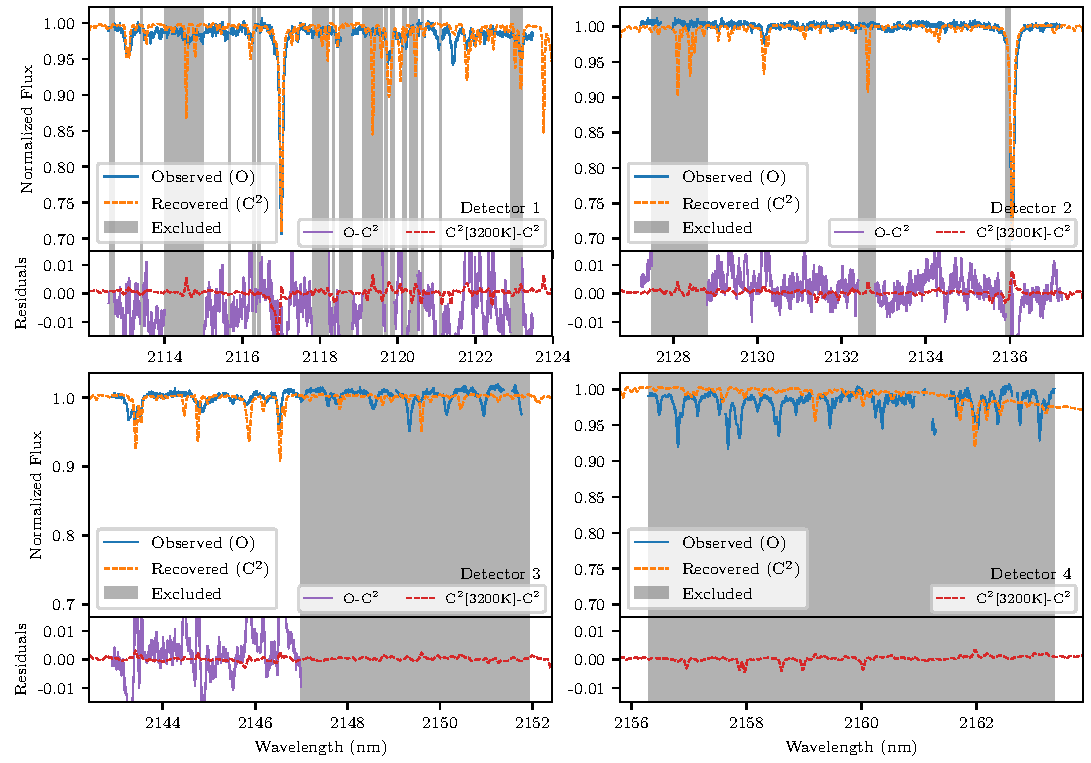
\includegraphics[width=0.8\hsize]{images/fig6.pdf}
    \caption{Comparison between the observed {HD 211847} spectrum (blue) and the best fit synthetic binary model (orange dashed) for each detector. The bottom section of each panel shows the residuals between the parts of the observation used in the \(\chi^2\) fit and recovered binary model (\(\rm O-C^2\)) in purple. The red dashed line shows the difference between the recovered binary model and the binary model with the exact same parameters except for the estimated companion temperature of 3200~K (\(\rm C^2[3200K]- C^2\)). The grey shading indicated the wavelength regions where masking has been applied. The thinner masked regions that match with cuts in the observed spectra are where the centres of deep (>5 per cent) telluric lines that have been masked out are.}
    \label{fig:visualinspection-hd2118471}
\end{figure*}

\subsection{Companion injection-recovery}
\label{subsection:injection-recovery}
To determine the detection limits for this method we employ an injection-recovery approach. We take the observed spectra and inject onto them a synthetic companion, at the absolute flux ratio to which it would have been added to a synthetic host with the same parameters. The injected companion RV is set to 100\kmps{} so that the companion lines are well separated from the lines of the host. This separation chosen is slightly larger than what we have with our observations, \(rv_2\) given in Table~\ref{tab:observations}.

We restrict the search space by fixing the host parameters \(T_{\textrm{eff}_1}\) and \(\rm logg_1\) to those recovered fitting the non-injected spectra by a single component model. The wavelength masking is used to reduce the level of mismatch between synthetic and observed spectra.

We apply the recovery method developed above on the injected spectrum, leaving only the companion \(T_{\textrm{eff}_2}\) and \({rv}_2\) parameters free, to recover the injected companion. We repeated this for injected companions with temperatures below 5000~K.

We also perform the injection-recovery with synthetic host spectra, representing each target. The wavelength range of the synthetic spectra used for this is three sections interpolated to 1024 values in the wavelength span of detectors 1, 2, and 3. For each section, Gaussian noise is added at the level measured in the corresponding detector for the in the observation of the target being represented.

In Fig.~\ref{fig:injection-recovery} we show the results of the injection-recovery on {HD 30501}. The blue dots represent the recovered companion temperature when injected into real observations, while the orange triangles represent injection into a synthetic host. Error bars of \(\pm100\)~K are included to indicate the grid size, and do not come from the recovery itself. The black dashed diagonal is the temperature 1:1 relation, where a correctly recovered companion should lie.

The grey shaded region indicates the \(\pm1000\)~K temperature range explored for the injection-recovery of the companion. This shows how the bounds of the grid are recovered at low temperatures.

For {HD 30501} the injection onto synthetic and observed spectra produce similar results. At temperatures above 3800~K in both the real and synthetic the injected companion is recovered within 100~K. For injected companion temperatures below 3800~K the temperature recovered is systematically higher than the injected value. This indicates that the companion is not correctly recovered and is affected by the added noise. We determine this temperature to be the upper temperature limit for the recovery. For the other stars we could not conclude on the upper limit due to spectral mismatch issues. In these cases we use the results from the synthetic injection to derive a temperature recovery cut-off for each target, each simulated with the closest host star spectrum.

In Fig.~\ref{fig:injection_shape} we show the minimum \(\chi^2\) for each companion temperature in the recovery grid. We do this for 7 different injected companion temperatures between 2500 and 4500~K. For the higher temperature companions, the \(\chi^2\) is parabolic in shape, recovering the correct temperature, as expected. At lower temperatures there is a strong asymmetry in the \(\chi^2\) with it flattening out on the lower temperature side.
The 1-, 2-, 3-\(\sigma\) values (with 2 degrees of freedom) of 2, 6 and 11 above the minimum \(\chi^2\) are not shown in the bottom panel of Fig.~\ref{fig:injection_shape} which is a close-up around the minimum \(\chi^2\) as are indistinguishable in the top panel due to the \(\chi^2\) y-scale. The black vertical line indicates the 2300~K temperature limit of the PHOENIX-ACES models.


\begin{figure}
    \centering
    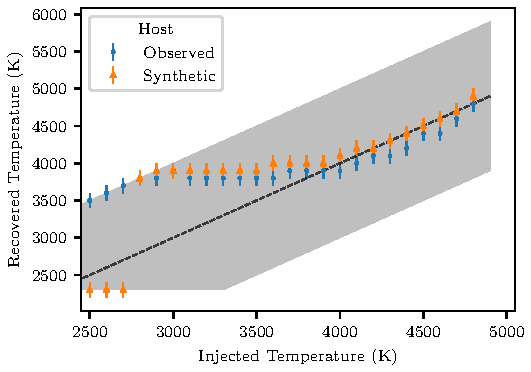
\includegraphics[width=0.95\hsize]{images/fig7.pdf}
    \caption{Result of simulated injection-recovery of synthetic companions on {HD 30501}. The blue dots and orange triangles indicate the recovered companion temperature for the observed and synthetic spectra respectively. The \(\pm100\)~K error bars are the grid step of the synthetic models. The black dashed diagonal shows the 1:1 temperature relation. The grey shaded region indicates the \(\pm1000\)~K temperature range explored. Gaussian noise added to the synthetic spectra was derived from the observed spectra.}
    \label{fig:injection-recovery}
\end{figure}


\begin{figure}
    \centering
    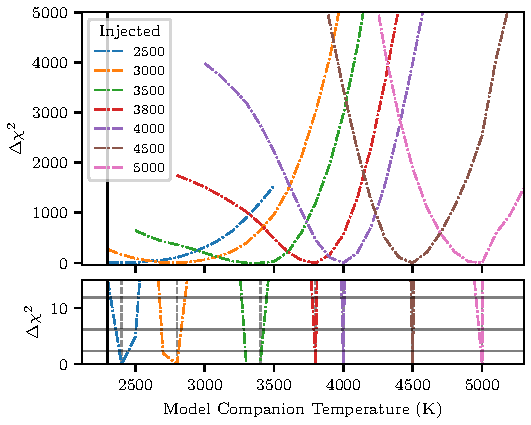
\includegraphics[width=0.95\hsize]{images/fig8.pdf}
    \caption{(top) Companion temperature verses \(\chi^2\) for simulations with different injected companion temperatures. Other fixed parameters for these fully synthetic simulations was \(T_{\textrm{eff}_1}=5200\)~K, \(\textrm{logg}_1=4.5\), \(\textrm{logg}_2=5.0\), and both [Fe/H] = 0.0. A fixed Gaussian noise corresponding to a SNR of 300 was used.
        (bottom) A close up view of \(\chi^2\) < 15. The three horizontal grey lines indicate the 1, 2, 3 sigma with 2 degrees of freedom. The vertical dotted lines indicate the location of the minimum \(\chi^2\) recovered for each companion. The black solid vertical in both panels shows the 2300~K cut-off of the PHOENIX-ACES models}
    \label{fig:injection_shape}
\end{figure}

%!TEX root = ../nir_companions.tex
\begin{table}
       \centering
  \begin{threeparttable}
     
       \caption{Upper mass limits of target companions assuming a companion logg = 5.0. Masses are derived from \citet{baraffe_new_2015} evolutionary models using \(T_{\textrm{eff}}\) and logg. The flux ratio \(\rm F_2/F_1\) is  the absolute flux ratio between the cut-off temperature and the target host star.}
      
        \begin{tabular}{l c c c}
            \toprule
            Target & \(T_{\textrm{eff}}\) cut-off (K) & \(\rm F_2/F_1\) & Mass limit ($\rm M_{jup}$)\\
            \midrule
            {HD 4747}     &  3900 & 0.084 & 598 \\ 
            {HD 162020} & 3900 & 0.147 & 598 \\
            {HD 167665} & 3800 & 0.054 & 560 \\
            {HD 168443} & 4000 & 0.094 & 618 \\
            {HD 202206} & 3900 & 0.075 & 598 \\
            {HD 211847} & 3900 & 0.079 & 598 \\
            {HD 30501}   & 3800\tnote{a} & 0.106 & 560 \\
            \bottomrule
        \end{tabular}
        \label{tab:mass_limits}
        \begin{tablenotes}[flushleft]
            \small
                \item [a] {From observed spectra }
        \end{tablenotes}
  \end{threeparttable}

\end{table}




Using the temperature cut-off values, we derive an upper mass limit for the companions around our stars using the~\citet{baraffe_new_2015} evolutionary models, finding the closest point matching the spectral temperature cut-off and \(\rm logg=5.0\). These values are given in Table~\ref{tab:mass_limits} and are between 560 and 618 \(\rm M_{Jup}\). The flux ratio between the cut-off and the host star are also provided for, being between 5 and 15 per cent in this wavelength span.


\section{Discussion}
\label{sec:discussion}
The spectral differential and the synthetic recovery methods attempted here were both unsuccessful in a detection of the BD companion spectra.  The upper mass limits of \(600^{+20}_{-40}\) we set for these companions is very high, roughly six times higher then the BD mass limit \(\sim\)80--90~\(\rm M_{Jup}\).
We discuss potential reasons and solutions for these poor results below, list the lessons learned in this exploratory study {of this dataset}, and provide some guidance for any future attempts with these methods.

\subsection{Synthetic recovery limitations}
\label{subsec:limitations}
In this section we discuss some of the limitations from this synthetic binary method and some options to overcome some of these.

\subsubsection{Mismatch in synthetic models}
\label{subsubsec:mismatch}
We believe the spectral mismatch between the observation and synthetic spectra is the main cause of the unsuccessful companion detection with the $\chi^2$ method with several strong lines in the model not observed in the spectra. This impacts the recovery in two ways; the spectral mismatch causes the \(\chi^2\) values to be large in general, but also causes the companion temperature to be pushed to higher temperatures, up to the constraints allowed by the grid.

In our examples the logg and metallicity of the synthetic models are held fixed, leaving only temperature to vary. The temperature impacts the synthetic spectral models in two main ways: the flux level of the continuum; and the number and strength of the absorption lines. In the binary model the contributions from the individual components is scaled by the flux ratio. If the temperature of the companion increases then the flux and radius of the companion increases. The contribution of the companion to the binary model increases and the flux ratio \(\rm F_1/F_2\) decreases. This effectively makes the lines of the spectrum of the host component relatively smaller in the normalized binary model spectrum. Due to the large initial mismatch of synthetic spectral lines of the host, a decrease in relative strength of the host lines decreases the \(\chi^2\) value, and is a better ``match'' to the observation. This causes the recovered temperature of the companion to be much higher than expected. If the companion temperature grid is allowed to extend it will recover a companion with a temperature >2000~K above the expected temperature. The \(\chi^2\) approach is dominated by reducing the mismatch in the spectrum of the host rather than actually detecting the spectra of the companion. When preforming the simulations in Sect.~\ref{subsec:simulated_binaries} there is no spectral mismatch between the simulation and the models, hence they do recover the correct host spectra and get closer values for the companion.

{To specifically check that the mismatch was not due to errors in our reduction we obtained the final spectral atlas of {10 LEO} from the CRIRES-POP archive, fully reduced and telluric corrected~\citep{nicholls_crirespop_2017}. Comparing the spectrum of {10 LEO} to a PHOENIX-ACES model with the corresponding parameters \(T_{\textrm{eff}_1}=4800\)~K, logg=3.0, [Fe/H] = 0.0 and convolved to R=90\,000,  similar line mismatches are observed. For 10 LEO, there is more spectral lines that agree with the model, but in the region of our observations between 2110--2160~nm there are deep lines in the model that are not observed, lines that have significantly different strengths, lines observed that are not modelled whilst other lines `appear' to be offset in wavelength, at the same positions observed in the work presented here. This indicates that the mismatch is not specific to our reduction only and that there is still room for improvement in synthetic models around 2100~nm.}

{Other works have also indicated regions or specific lines in which synthetic models did not reproduce all of the spectral features seen in stellar spectra~\citep[e.g.][]{delburgo_physical_2009, bonnefoy_library_2014, passegger_spectroscopic_2016, rajpurohit_spectral_2016}.}

\subsubsection{Line contribution of faint companions}
\label{subsubsec:line_contributions}
We calculate the line depths of the synthetic companion spectra to determine the SNR levels required to detect the lines of the binary companions.
One thing easy to overlook when attempting to detect the binary companion at low flux ratios is the actual contribution of the spectral lines of the companion.
The flux ratio of the continuum for our most promising target is \(\rm F_2/F_1\)\(\sim\)1 per cent with the other targets having an expected flux ratio 0.5 per cent, and some well below. The spectral lines of the individual components which are the features we are trying to detect with the binary model, have depths on average around 10--20 per cent of their respective continua,  at-least between 2110--2160~nm. In effect, the companion line features have a depth \(\ll\) 1 per cent relative to the continuum of the combined spectra.

In Table~\ref{tab:line_contributions} we calculate some properties of the spectral lines in the PHOENIX-ACES library between 2110--2160~nm. We count the number of spectral lines (\emph{no.\ lines}) deeper than 5 per cent, and take the average depth (\emph{avg.\ depth}) of these lines. The contribution \emph{cont.\ depth} of the companion lines to a combined spectrum accounts for the flux ratio between the two components. Here we use a Sun-like host with \(T_{\textrm{eff}_1}=5800\)~K. This simplified combination neglects the continuum shapes of both spectral components and uses the average flux ratios for this wavelength range. The PHOENIX-ACES spectra in the temperature range of 2500--5000~K shown in Fig.~\ref{fig:comp_spectra} can be used to get a visual indication of the line density and depth measured here.

There are more lines >5 per cent deep for the lower temperature spectra, with 360--460 lines in this wavelength range, to be compared with the 31 deep absorption lines found in a Sun-like spectrum. The average line depth of these lines is also larger than the Sun-like spectrum, around twice as deep. However, when combined, the contribution of the companion lines is 1--2 orders of magnitude smaller than the hosts lines due to the low continuum flux ratios.

For example, with the synthetic model for the companion of {HD 211847}, the average contributions of lines >5 per cent become only 0.3 per cent deep in a binary with the Sun-like spectrum. For a companion with a temperature of 2300~K (the lower PHOENIX-ACES temperature limit) the deepest lines contribute lines around 0.1 per cent.

The SNR of the observed spectra is between 150--350, which is below the SNR of 323 needed for the detection of the low-mass star companion of {HD 211847} with temperature 3200~K and logg 5.0. For our other targets with BD companions at and below the PHOENIX-ACES temperature range, we would need observed SNR >800 to detect the individual spectral lines of the companion. With the SNR increasing with \(\sqrt{N}\) this would require the observational time for each target to be increased by a factor of \(\sim\)10--64.
{This is in line with the recent detection of the spectrum of a non-transiting giant planet by~\citet{piskorz_evidence_2016} which utilized nIR spectra with SNR > 2000, from 1--3 hours of observation each.}

Our non-detection of binary companions with low flux ratios is consistent with results from other works. For example~\citet{nemravova_xtauri_2016} performed extensive spectral analysis of a quadruple-star system {$\xi$ Tauri} using 227 spectra in 3 different wavelength bands. Of the four stars in the system they were unable to detect the spectral component of the one which had a luminosity ratio below 1 per cent. {The secondary detection in optical spectra using spectral matching of KOI was also only able to reach flux ratios of 1 per cent~\citet{kolbl_detection_2015}.}

%!TEX root = ../nir_companions.tex

\begin{table}
        \small
    \begin{threeparttable}[b]

   \caption{Contribution of synthetic lines within 2110--2160~nm of synthetic PHOENIX-ACES spectra to a binary model. \(F_{2}/F_{1}\) is the continuum flux ratio between a spectrum with the given \(T_{\textrm{eff}}\) and logg and a Sun-like spectrum with \(T_{\textrm{eff}}=5800\), logg = 4.5 (right most column). \emph{No.\ lines} is the number of spectral lines deeper than 5\% from the continuum of the individual spectra while \emph{avg.\ depth} is the mean depth of those lines. \emph{Cont.\ depth} is the average contribution, or depth, of these lines in the combined spectrum of a binary with a Sun-like spectrum. The SNR is signal-to-noise level required to have Gaussian noise \(\sigma\) =1/SNR equal to the \emph{cont.\ depth} level in the binary model. All synthetic spectra used here have [Fe/H]=0.0.}
    
    \begin{tabular}{*7c}
        \toprule
        \(T_{\textrm{eff}}\) (K)  & \multicolumn{2}{c}{2300} & \multicolumn{2}{c}{3200} & 5800 (\(\rm F_1\))\\
        logg & 5.0 & 4.5  & 5.0 & 4.5 & 4.5 \\
        \midrule
        \(F_2/F_1\) & 0.006 & 0.019 & 0.029  & 0.091 & 1.000 \\  
        % {>2\%}  & no. lines & 470 &  463 & 414  & 444 & 111 \\
        % & avg.\ depth & 0.20 & 0.23 & 0.10  & 0.12 & 0.04 \\
        % & cont. depth \tablefootmark{a} & 0.0012 &  0.0043 & 0.0028 &  0.0100 &  0.0333\tablefootmark{b} \\ 
        % \midrule
        no.\ lines & 464 & 463 & 365  & 413 & 31 \\
        avg.\ depth & 0.2  & 0.23& 0.11 & 0.12 & 0.10 \\
        cont.\ depth\tnote{a} &  0.0012 & 0.0043 &  0.0031 & 0.0100&  0.0833\tnote{b} \\ 
        SNR  & 833 & 232 & 323  & 100 & 12 \\ 
        %  SNR\(\rm _N\)  & 39 & 11 & 17  & 5 & 2 \\ 
        \bottomrule
    \end{tabular}
    \begin{tablenotes}
        \item [a] avg.\ depth \(\times~ \rm F_2 / (F_1 + F_2)\), where \(F_1\) is the component in the far right column.
        \item[b] avg.\ depth \(\times~ \rm F_1 / (F_1 + F_2)\), where \(\rm F_2\) is for the companion with \(T_{\textrm{eff}}\)=3200, logg=4.5.
    \end{tablenotes}
    \end{threeparttable}
    \label{tab:line_contributions}
\end{table}

\subsubsection{\(\chi^2\) asymmetry}
\label{subsubsec:chi2_assymetry}
In Fig.~\ref{fig:injection_shape} we showed that the shape of the recovered \(\chi^2\) becomes asymmetric when dealing with companion temperatures below around 3800~K. A visual inspection of the spectra reveals the likely cause. In Fig.~\ref{fig:comp_spectra} we show the corresponding spectra between 2111--2165~nm. As the temperature decreases the strongest lines become less prominent, disappearing progressively among the other many small lines that appear at lower temperatures. Hence there are no strong companion lines to easily distinguish one temperature from another. In the flatter part of the \(\chi^2\) curves several low temperature companions are equally well fitted to the simulation/observation.

Figures~\ref{fig:injection-recovery} and~\ref{fig:injection_shape} show different recovered temperatures but both agree above 3800~K. A higher companion temperature is recovered between 2800 and 3800~K, where as in Fig.~\ref{fig:injection_shape} a lower temperature is recovered. This is probably due to a combination of the noise added, and the asymmetries of the \(\chi^2\) lines. Figure~\ref{fig:injection-recovery} uses the noise level from the observed spectrum while Fig.~\ref{fig:injection_shape} has a SNR of 300.
This large asymmetry can also explain the jump observed in the synthetic recovery temperature around 2700~K in Fig.~\ref{fig:injection-recovery}.

The asymmetry also causes an asymmetry in the \(\chi^2\) error bars which can be seen in the bottom panel of Fig.~\ref{fig:injection_shape}. For instance the recovered value and 1-\(\sigma\) error bars on the 3000~K injected companion is \(2800 ^{+20}_{-100}\), with an asymmetric error bar skewed towards lower temperatures.

The bump observed at 5100~K in the \(\chi^2\) curves is due to a discontinuity in the PHOENIX-ACES modelling. The ``reference wavelength defining the mean optical depth grid'' is changed at 5000~K~\citep[][Sect. 2.3]{husser_new_2013}. Care needs to be taken if trying to detect a companion near this temperature.

\begin{figure}
    \centering
    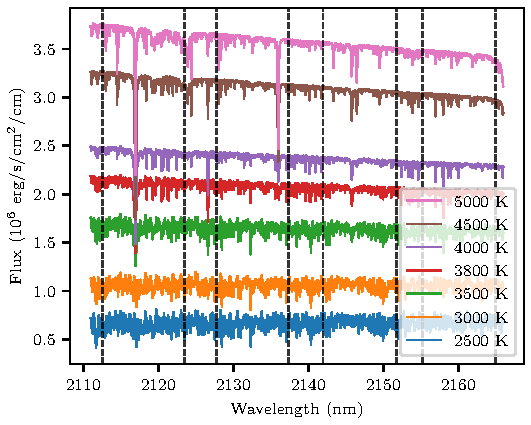
\includegraphics[width=0.95\hsize]{images/fig9.pdf}
    \caption{PHOENIX-ACES spectra for temperatures between 2500 and 5000 K, corresponding to to the same lines in Fig.~\ref{fig:injection_shape}. The flux units are the native units of the PHOENIX-ACES spectrum, (\(\rm erg\,s^{-1}\,cm^{2}\,cm^{-1}\)), and have not been scaled by the stellar radii. All spectra have a \(\rm logg=5.0\) and \(\rm [Fe/H]=0.0\). The vertical dotted lines indicate the edges of the CRIRES detectors.}
    \label{fig:comp_spectra}
\end{figure}

\subsubsection{Component RV separation}
\label{subsubsec:rv_seperation}
Another factor which could contribute to an unsuccessful detection is the RV separation between the host and companion, \(rv_2\). Estimates for our observations are given in the last column of Table~\ref{tab:observations}. If \({rv}_2\) is small compared to the line width, then all the same lines of both components will be blended. This is indeed the case for {HD 4747}, {HD 211847}, and {HD 202206} with expected \(|{rv}_2| < 2\)\kmps{}, {due to poor observational planning}. This may have contributed to the lack of recovery with both components of the binary model attempting to fit the same features. This may even cause correlation between the parameters of the two components. The RV separation of the two components changes with orbital phase. Having multiple spectra of the same target distributed in phase may allow the RV of the spectral components to be better recovered~\citep[e.g.][]{czekala_disentangling_2017, sablowski_spectral_2016}.
{Similarly~\citet{kolbl_detection_2015} were unable to detect companion stars within 10\kmps{} of the host using optical spectra}.

\subsubsection{Wavelength range}
\label{subsubsec:wavelenght_range_limitation}
{The wavelength range for these observations was chosen specifically due to the location of the \textit{K}-band telluric absorption window. This was to reduce telluric contamination present in the spectra intended for the spectral differential technique. The wavelength range is also very narrow (\(\sim\)50~nm) and was set by the CRIRES instrument. The small number and inconsistent distribution telluric lines made the wavelength calibration method using the telluric lines difficult in some regions (specifically detectors 2 and 3). For the $\chi^2$ fitting of faint companions this narrow wavelength region is likely not the best choice given the small number of stellar lines and unique spectral features of the companion. For example~\citet{passegger_fundamental_2016} use 4 different wavelength regions with lines from different species to fit PHOENIX-ACES models to M-dwarf stars while other studies aiming to detect planetary companions choose wavelength regions which contain strong planetary absorption features such as the absorption of CO and H$_2$O near 2.3 $\mu$m~\citep[e.g.][]{dekok_detection_2013, brogi_carbon_2014}.
Applying the binary fitting to a different wavelength region with lines more sensitive to stellar parameters for both stars and BDs, as well as using a larger wavelength range (i.e.\ provided by the cross-dispersion on CRIRES+~\citep{dorn_crires_2016}), should improve the recovery results of the technique presented here. We note that if the wavelength range is increased by taking separate observations at different wavelengths, not covered by a single exposure, then changes in the RV of both components between the different wavelength observations will need to be accounted for.}

\subsubsection{The {BT-Settl} models}
\label{subsubsec:BT-Settl}
We note that the PHOENIX-ACES models are not the only spectral libraries available with the other notable library considered for this work is the {BT-Settl} models~\citep{allard_model_2010,allard_btsettl_2013,baraffe_new_2015}. The included modelling of dust and cloud formation, as well as hydro-dynamical modelling atmospheric mixing/settling for atmospheres with \(T_{\textrm{eff}}\) below \(\sim\)2600~K, make the {BT-Settl} models valid across the regime from stars to BDs as cool as 400~K. As the {BT-Settl} models are suitable to model the atmospheres of the brown dwarfs they would be useful for the companion recovery technique developed here. However, as shown in Sect.~\ref{subsection:results-hd211847} and~\ref{subsection:injection-recovery}, we were unable to successfully recover the 155 \(\rm M_J\) (\(T_{\textrm{eff}}\sim\)3200~K) low mass star companion of {HD 211847} and derived a temperature upper limit for our methodology of around 3800~K. These are both well above the 2300~K cut-off of the PHOENIX-ACES models and for the onset of dust- and cloud-formation phenomena, at 2600 K.

Fig.~\ref{fig:hd211847-models} shows again the minimum \(\chi^2\) solution for detector 1 of the second {HD 211847} observation, this time including the {BT-Settl} solution with the same parameters. Although the PHOENIX-ACES and {BT-Settl} models differ slightly they both have a large spectral mismatch to the observations. As such, we did not use the {BT-Settl} models for the simulation and results above as we did not see any special advantage in using them.

The ease of access to find, download, and use PHOENIX-ACES spectral library, available in the fits file format, compared to older {BT-Settl} libraries is another reason for the current favoured use of the PHOENIX-ACES library.

Although the newer generations synthetic spectral models are improving and match the overall spectral energy distribution reasonably well there are still regions in the \textit{H}- and \textit{K}-band where there is room for improvement~\citet{rajpurohit_spectral_2016}. The spectral mismatch in the region studied here is still too large for spectral recovery of companion brown dwarfs. In the nIR we have compounding problem: the model input physics of sub-stellar temperatures and chemistry combined with the general difficulty of the nIR.

\begin{figure}
    \centering
    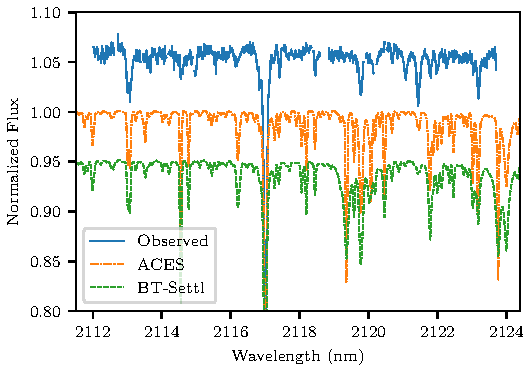
\includegraphics[width=0.95\hsize]{images/fig10.pdf}
    \caption{Detector 1 spectrum for {HD 211847} (blue) alongside the PHOENIX-ACES (orange dash-dot) and {BT-Settl} (green dashed) synthetic spectra for the host star only, with parameters \(T_{\textrm{eff}}=5700\)~K, \(\rm logg=4.5\) and \(\rm [Fe/H]=0.0\). Both synthetic models have been normalized and convolved to \(\rm R=50\,000\). There is a 0.05 off-set between each spectrum}
    \label{fig:hd211847-models}
\end{figure}

\subsubsection{Impact of logg}
\label{subsubsec:logg}
Logg, a measure of surface gravity, is related to evolutionary state and the size of the star with smaller logg values usually indicating larger radii stars. This parameter has a large impact on the radius and flux ratio of the binary models. In the PHOENIX-ACES models a decrease in logg from 5.0 to 4.5 increases the models effective radius by \(\sim\)1.75 in the temperature range investigated here. This change in radius alone roughly triples (\(1.75^2\)) the absolute flux of the synthetic spectrum, neglecting any changes to the shape of the actual spectrum. Therefore, there are large jumps in the model flux ratios if the logg is allowed to vary, with lower logg values for the companion being favoured as the increased flux ratio decreases the mismatch of the host component to the observations. This large impact of logg on the spectral library absolute flux is one reason for keeping the logg of each component fixed in the \(\chi^2\) results presented in Sect.~\ref{sec:results}.

\subsubsection{Interpolation}
\label{subsubsec:interpolation}
It is common to interpolate between the synthetic spectral grids to fit and derive parameters in between the grid points~\citep[e.g.][]{nemravova_xtauri_2016, passegger_fundamental_2016}. Instead of interpolation~\citet{czekala_constructing_2015} use a spectral emulator to use Principal Component Analysis to create eigenspectra for the synthetic library and Gaussian processes to derive a probability distribution function of possible interpolation spectra to account for uncertainties in the interpolation required for high signal-to-noise spectra.

However, we did not incorporate any interpolation into the companion recovery at this stage. This could be something to be added in the future to refine the recovered parameters, and to help the transition between the grid logg values. Codes are readily available to perform spectral interpolation which could be utilized for this, two of them are \textsc{pyterpol}\footnote{https://github.com/chrysante87/pyterpol}~\citet{nemravova_xtauri_2016} and \textsc{Starfish}\footnote{https://github.com/iancze/Starfish}~\citep{czekala_constructing_2015}.

\subsection{Future implementation}
\label{subsec:future}
\subsubsection{High resolution instrumentation}
\label{subsubsec:highres}
The future of high resolution near- and mid- IR spectrographs is looking bright, with many new ground- and space-based instruments currently being developed. Notable examples include CARMENES (550--1710~nm, R=82\,000) which is now operational~\citep{quirrenbach_carmenes_2014}, while SPIRou (980--2350~nm, R=73\,500)~\citep{artigau_spirou_2014} and NIRPS (970--1810~nm, R=100\,000)~\citep{bouchy_nearinfrared_2017} are still being assembled and installed. The eagerly awaited \textit{JWST}~\citep{gardner_james_2006} will provide observations in both the near-IR (600--5300~nm, R=2700) and mid-IR (4900--28\,800~nm, R$\sim$1550--3250) regions without contamination from our atmosphere.

The upgrade of CRIRES to CRIRES+~\citep{dorn_crires_2016} will increase the wavelength coverage of a single shot capture by at least a factor of 3--5. This larger wavelength span would be extremely beneficial for the \(\chi^2\) performance of the spectral recovery method, increasing the number of useful lines and spectral features to be fitted with the models.

On the modelling side, there are continual improvements in atmospheric modelling and their associated synthetic spectral libraries: as seen with the evolution of the {BT-Settl} models~\citep{allard_btsettl_2013}. With additional physics and improved line lists and solar abundances~\citep[e.g.][]{asplund_chemical_2009,caffau_solar_2011}, the synthetic libraries are reaching a better agreement with nIR observations. An improved agreement between the nIR observations and synthetic spectra will be crucial to improve the performance of the spectral recovery technique presented here.

Although not successful with the CRIRES data used here, the instrumental stage is set to attempt these techniques presented here using the next-generation of high resolution spectrographs. The lessons learned in this analysis need to be taken into account in order to achieve the best chance of a successful detection.


\subsection{Other techniques}
We note that there are many other disentangling techniques to separate mixed spectra of binary systems,~\citep[e.g.][]{hadrava_disentangling_2009}. These require more than two observations, with  \(n+1\) observations used to set up a system of linear equations to solve for \(n\) spectral components~\citep[e.g.][]{simon_disentangling_1994,czekala_disentangling_2017, sablowski_spectral_2016}. These methods are ideal for many well spaced observations. For example the ideal situation for the SVD method of~\citet{sablowski_spectral_2016} is homogeneous samples of at least half the period, to identify the moving spectral components.
{Recently the cross-correlation and maximum-likelihood techniques~\citep[e.g.][]{lockwood_nearir_2014, piskorz_evidence_2016} have been successful in detecting the faint companion spectra of giant planets using several spectra with very-high SNR (>2000) obtained with longer observational time (1--3 hours) each taken across the full orbital range.} The few, short and insufficiently separated observations we analyse here are not suitable to apply these advanced techniques and are beyond what we have attempted here.

{ The recent work of~\citet{piskorz_evidence_2016} use a PCA technique to correct for the telluric spectra by applying it to several (number not specified) AB nodding pairs over their 60--180 minute integration time. We are uncertain if this technique would work as effectively on our observations due to our shorter integration time (24 minutes) would have less telluric variation present across the 8 nod spectra. A recent comparison of three telluric correction methods, \textsc{Molecfit} and \textsc{TelFit} and {TAPAS} to the standard star method by (Ulmer-moll et al. (in preparation)) %~\cite[][in prep.]{ulmer-moll_telluric_2018}
 found that all three synthetic models preform better at correcting for atmospheric H$_2$O compared to the standard star method with \textsc{Molecfit}, being a more complete tool, preforming slightly better over TAPAS.}


\section{Conclusions}
\label{sec:conclusions}
This work explored a spectral recovery technique to detect the faint spectra of stellar companions in blend spectra, using high resolution near-infrared spectra. 

For the spectral recovery the host-companion RV separation should also ideally be greater then the FWHM to avoid blended lines. The spectral mismatch between models and reality in the nIR negatively affects the performance of the synthetic recovery technique on the observed spectra. With all these effects we are unsuccessful in the detection of the nIR spectra of BD companions,  with the mass upper-limits set at \(\rm 600~M_{Jup}\) from the synthetic recovery technique.

This work highlights many of the difficulties when dealing with the spectral recovery of nIR spectra. The obstacles to overcome are the data reduction of nIR CMOS detectors, that are not yet at the level of visible CCDs, along with a precise telluric correction and wavelength calibration (two interrelated aspects, as thoroughly discussed). Another important aspect is the mismatch between nIR high-resolution spectra and the observed spectra. In spite of the continuous effort of the modelling community, our work, along with several cited contemporary ones, shows that this mismatch is still one of the main factors preventing us from performing spectral recovery in the nIR.\@ This work highlights that this is a compound problem for Brown Dwarfs, for which the spectral models are worse informed due to lack of observations at high-resolution.

Other than the improvement of the spectral models, the observing community can increase their odds of success by paying attention to the scheduling of observations and the wavelength domains to explore. Our work shows that observing in the areas of lower telluric absorption, as is frequently done, is not a guarantee of success due to the scarcity of deep lines in cold objects. Moreover, due to the mismatch between models and observations, the ability to obtain a first spectra before settling on a wavelength range, or changing settings on the fly, is extremely useful for the success of these campaigns.

We hope that this work can act as a guide for the planning of future observations of targets with faint BD and planetary companions with the upcoming generation of high resolution spectrographs in the near- and mid-infrared such as CRIRES+ and JWST observations.


\section*{Acknowledgements}
This work was supported by Funda\c{c}\~ao para a Ci\^encia e a Tecnologia (FCT) (Portugal) research grants through national funds and from FEDER through COMPETE2020 by the following grants: UID/FIS/04434/2013, \&  PTDC/FIS-AST/1526/2014, \& PTDC/FIS-AST/7073/2014, \& POCI--01--0145-FEDER--016886, \& POCI--01--0145-FEDER--007672, \& POCI--01--0145-FEDER-016880, \& POCI--01--0145-FEDER-032113.
J.J.N. acknowledges support from FCT though the PhD::Space fellowship PD/BD/52700/2014.
P.F., N.C.S. acknowledge support from FCT through Investigador FCT contracts IF/01037/2013CP1191/CT0001, \& IF/00169/2012/CP0150/CT0002, \& IF/00028/2014/CP1215/CT0002, \& IF/01312/2014/CP1215/CT0004.
This work made use of \textsc{PyAstronomy}\footnote{Available at \href{https://pyastronomy.readthedocs.io}{https://pyastronomy.readthedocs.io}} and many other open source and under-credited software packages numpy, scipy, astropy, Starfish to name a few.
This research has made use of the SIMBAD database, operated at CDS, Strasbourg, France.

%%%%%%%%%%%%%%%%%%%% REFERENCES %%%%%%%%%%%%%%%%%%
% The best way to enter references is to use BibTeX:
\bibliographystyle{mnras}
\bibliography{nir_companions}

%%%%%%%%%%%%%%%%% APPENDICES %%%%%%%%%%%%%%%%%%%%%
\appendix

    % Table of estimates of parameters
    %!TEX root = ../nir_companions.tex
\begin{table*}
  %   \begin{threeparttable}[b]
        \small
        \centering
        \caption{Estimated flux ratios, orbital semi-amplitude and RV separation of the companion, given the companion mass (\(\textrm{M}_{2}\) or \(\textrm{M}_{2} \sin{i}\)) from Table~\ref{tab:orbitparams} and observation times from Table~\ref{tab:observations}.} 
        \begin{tabular}{l | c c c c c c c | c c c}%[hb]
            \toprule
            & Host& Companion &  Estimated  & Estimated &  Estimated & Estimated &  &    \\  % 2017
            Companion & M$_{K}$ & M$_{K}$ & \(\rm F_{2}/F_{1} \)   & \(\rm N_{2}/N_{1} \) (noise ratio) & \(\rm K_2\) &   \(\Delta RV\) & Phase coverage \\
            & & & \textit{K}-band     & & (\kmps{}) & (\,ms\(^{-1}\)) & (\%) \\
            \midrule
            {HD 4747}        & 3.82 & 14.17 & \(7\times10^{-5} \)   & 76 &  -10.65 & -  &  -  \\  % 2017
            {HD 162020}    & 4.10 & 23.36 & \(2\times10^{-8} \)   & 1615  &  -98.92\tnote{a} &  2344.24     & 0.28~~  \\  %
            {HD 167665}    & 2.60 & 13.21 & \(6\times10^{-5} \)   &  105    &  -14.47\tnote{a}  &   138.45     & 0.18~~  \\  %  -- \(2\times10^{-5} \)  best case based on age rage.
            {HD 168443b}  & 2.35 & 42.19 & \(1\times10^{-16} \)  &    \(1\times10^{8} \)   &  -64.65\tnote{a}&   257.16   & 0.035 \\ 
            {HD 168443c}  & 2.35 & 29.55 & \(1\times10^{-11} \)  &   \(4\times10^{5} \)     &  -18.05\tnote{a}  &   0.95   &  0.001 \\  %(c)
            {HD 202206}B  & 3.04& 21.63 & \(4\times10^{-8} \)  &   1586 &  -6.79 & 145.17   & 0.74~  \\  %(B)   % May2017
            {HD 202206}c   & 3.04& 45.63 & \(9\times10^{-18}\)   &     \(2\times10^{7} \) &   -2.50     &   0.67     &  0.15~  \\  %(B)   % May2017
            {HD 211847}B  & 3.50 & 8.40 &  0.011 &  14   & $-$1.85 & 3.88   & 0.09~  \\  %B % 2017
            {HD 30501}      & 3.96 & 10.38 & check 0.003  &  27  &  -16.12    &  1346.46      & 5.8~~  \\
            \bottomrule& & 
            \end{tabular}
    \begin{tablenotes}
        \item[a] {Maximum \(K_2\) only given \(M_2 \sin{i}\)}
      \end{tablenotes}
%    \end{threeparttable}
    \label{tab:estimatedparameters}
\end{table*}


    \section{Estimating companion parameters}
    In this appendix we detail how we calculate RV of the components and determine the flux ratio of our targets given their literature masses \(M_2\) or \(M_{2}\sin{i}\). We refer to these calculations as estimates as in some cases we only have the companions minimum mass.

    The estimated \(K_2\) for each companion is provided in Table~\ref{tab:estimatedparameters} while the RV for both components at the time of each observation is provided in Table~\ref{tab:observations}.



    {\bl The host companion contrast ratio is calculated from the magnitude difference. Magnitudes for the companion are interpolated from the Barraffe tables.
        
    A simple tool\footnote{Available at \url{https://github.com/jason-neal/baraffe_tables}} was created to calculate the flux ratio using the~\citep{baraffe_evolutionary_2003,baraffe_new_2015} evolution tables. Given the host star name, the companion mass and a stellar age it interpolates the available Baraffe tables to the companion mass and age specified. The host's name is used to query the {SIMBAD} database to obtain stellar properties, specifically magnitudes, to calculate the flux ratios. It can also work in reverse to estimate a companion mass when provided with a flux ratio.}

% Don't change these lines
\bsp{}	% typesetting comment
\label{lastpage}
\end{document}

% End of mnras_template.tex
